% !TEX root = diss.tex

\chapter{Interrogation of the Bell-Evans-Polanyi Principle: Investigation of
the Bond Dissociation Enthalpies Correlated with Hydrogen Atom Transfer Rate
Constants} \label{ch:bde}

\section{Introduction}

The Bell-Evans-Polanyi (BEP) principle is a conceptual framework that states,
for two closely related reactions, the difference in activation energy is
proportional to the difference in their enthalpy of
reaction.\cite{Bell1936,Evans1938,Dill2003} This is commonly expressed as the
linear free energy relationship (LFER): $E_a = E_0 + \alpha \Delta H$
(Equation~\ref{eq:bep}). Initially, the BEP principle was used as a simple
model to explain the Br{\o}nsted catalysis law, which states that the stronger
an acid is, the faster the catalyzed reaction will proceed.\cite{Bronsted1924}
A key assumption is made for the BEP principle: the position of the TS along
the reaction coordinate is the same for all reactions. The relationship can be
described schematically: the more stable the product, the lower the reaction
barrier, as seen in~\ref{fig:bep}.

\begin{figure}[!htbp]
  \centering
  
\includegraphics[width=0.7\textwidth]{figures/bep}
  \caption{Energy profiles for a series of related exothermic reactions
  illustrating the Bell-Evans-Polanyi principle.} \label{fig:bep}
\end{figure}

A modern utilization of the BEP principle is to estimate rate constants of
related reactions. This is a desirable, because as system size increases, ab
initio computational modelling becomes computationally challenging, or even
infeasible due to the exponential scaling of computational cost with system
size. Therefore, the main purpose of LFERs is to apply previous knowledge to
new systems and help develop insights. For example, much of our groups' work
focuses on studying simple protein models. By thoroughly investigating small
systems with ab initio approaches, it is possible to extrapolate the
fundamental concepts to large-scale systems. Furthermore, if one can establish
that there exists a LFER between activation energy and bond strength for a
specific model, then the difference in bond dissociation enthalpy (BDE) can be
used to estimated HAT reaction rates in a large-scale protein system.

In application of the BEP principle in HAT reactions, plots of the logarithm of
the rate constant ($k_H$) against BDEs are commonly used: $\log(k_\mathrm{H}) =
\alpha \Delta H + constant$. For HAT reactions involving abstraction by \cumo,
the enthalpy of reaction ($\Delta H$) is directly related to the strength of
the breaking bond: $\Delta H =$ BDE(\ch{C-H}) $-$ BDE(\ch{CumO-H}). If the
relationship holds for a series of related HAT reactions, then BDEs should
correlate with the activation energy. It would then stand that an increase in
bond strength represents a destabilization in the TS complex, and thus a
decrease in reaction rate. This concept is also important for the work in
Chapter~\ref{ch:hat}, where the interaction of non-redox active metal cations
results in an increase in effective bond strength, and decrease in rate
constant. It is also important to note that if the BEP principle breaks down
for reactions that appear related, then additional physico-chemical factors,
such as non-covalent binding (\emph{viz.} Chapter~\ref{ch:arrhenius}), or
stereo-electronics may be influencing the reaction barrier.

An interesting application of the BEP principle is the work of
\citet{Pratt2003}, in which the free radical oxidation of unsaturated lipids
was examined. They studied the correlation of theoretically determined allylic
or benzylic C-H and \ch{C-OO^.} bond strengths with experimentally-measured HAT
rate constants and \ch{O2} addition rate constants, respectively. BEP plots
($\log k$ vs. BDE) for a large range of polyunsaturated fatty acid models show
good correlation ($R^2 = 0.92$) for \ch{C-OO^.} bonds examined, and reasonable
correlation ($R^2 = 0.82$) for \ch{C-H} bonds. This demonstrates that BDEs may
directly impact the reaction barrier height, in line with the BEP principle.
Additionally, these results provide the important ability to predict rate
constants for HAT and oxygen addition reactions related to unsaturated lipid
models, by means of calculating BDEs. Another area of research in which the BEP
principle is often applied is heterogenous catalysis.\cite{Panov2015}

There is a significant gap in the literature on the BEP principle: there are no
criteria for how broadly the BEP principle can be utilized. In fact, the
theoretical validity of the BEP relationship has come into question, and a call
has been made to theoreticians for a detailed analysis of the BEP
principle.\cite{vanSanten2010} In this work, I explore this issue. In order to
achieve this, I have studied HAT reactions involving the abstraction of C-H
bonds by \cumo\ under the same experimental conditions, for which many rate
constants have been published.\cite{Bietti2010, Bietti2011, Pischel2001,
Salamone2011, Salamone2012, Salamone2012a, Salamone2013, Salamone2015}
Additional unpublished rate constants have been provided by our experimental
colleagues in Rome. The substrates of interest are diverse in nature and
include branched and cyclic alkanes, linear and cyclic amines and ethers, and
substrates with allylic or benzylic \ch{C-H} bonds. The BDEs for these
substrates range from $\sim$76--100 \kcalmol. The experimentally determined
rate constants are listed in Appendix~\ref{ap:bde},~\ref{tab:expt-bde}.

The above studies, as well as many others, have used \cumo\ and the closely
related $t$-butoxyl radical (\ch{$t$-BuO^.}) as models for reactive
oxygen-centred radicals in studying oxidative damage of
biomaterials,\cite{Adam1998, Adam2002, Jones2003} as well as in studying the
mechanism and efficiency of antioxidants.\cite{MacFaul1996, Valgimigli1996,
Valgimigli1999, Jovanovic1999, Sortino2003} Using these radicals to study
biomolecular oxidation has an important caveat: The fundamental chemistry of
these radicals is less well understood than is often assumed. \cite{Tanko2001,
Finn2004, Salamone2011b}

The BDE of \ch{CumO-H} is 106.7 \kcalmol, a value that is larger than all the
\ch{C-H} bonds studied herein.\bibnote{Calculated using the ROCBS-QB3 composite
method.} Therefore, HAT reactions involving \cumo\ and the organic substrates
of interest are all exothermic on the order of 5--32 \kcalmol. Hammond's
postulate\cite{Hammond1955} states that the the transition states for these HAT
reaction should most closely resemble the reactants in structure (i.e.  an
early TS), and the BEP $\alpha$ values should all be less than
0.5.\cite{Russell1973} If the BEP principle holds as a LFER, the substrates
should be considered as if the BDEs were controlled by substituent effects. For
example, if one considers methane as the reference \ch{C-H} bond model, the BDE
of toluene should reflect the effect of replacing one hydrogen with a phenyl
group. This is also the basis for schemes that utilize group additivity to
predict molecular heats of formation.\cite{Benson1976}

Considering this group additivity-like approach, our colleague in Rome, Massimo
Bietti, hypothesized that there should exist two general BEP relations for C-H
bond: one in which the incipient radical is delocalized into a $\pi$-system
(benzylic or allylic), and one in which the remaining alkyl radicals are
largely localized. Plotting the experimental rate constants against literature
BDEs (\ref{fig:bep-expt}) there appears to be evidence for the two BEP
relations.

\begin{figure}[!htbp]
  \centering
  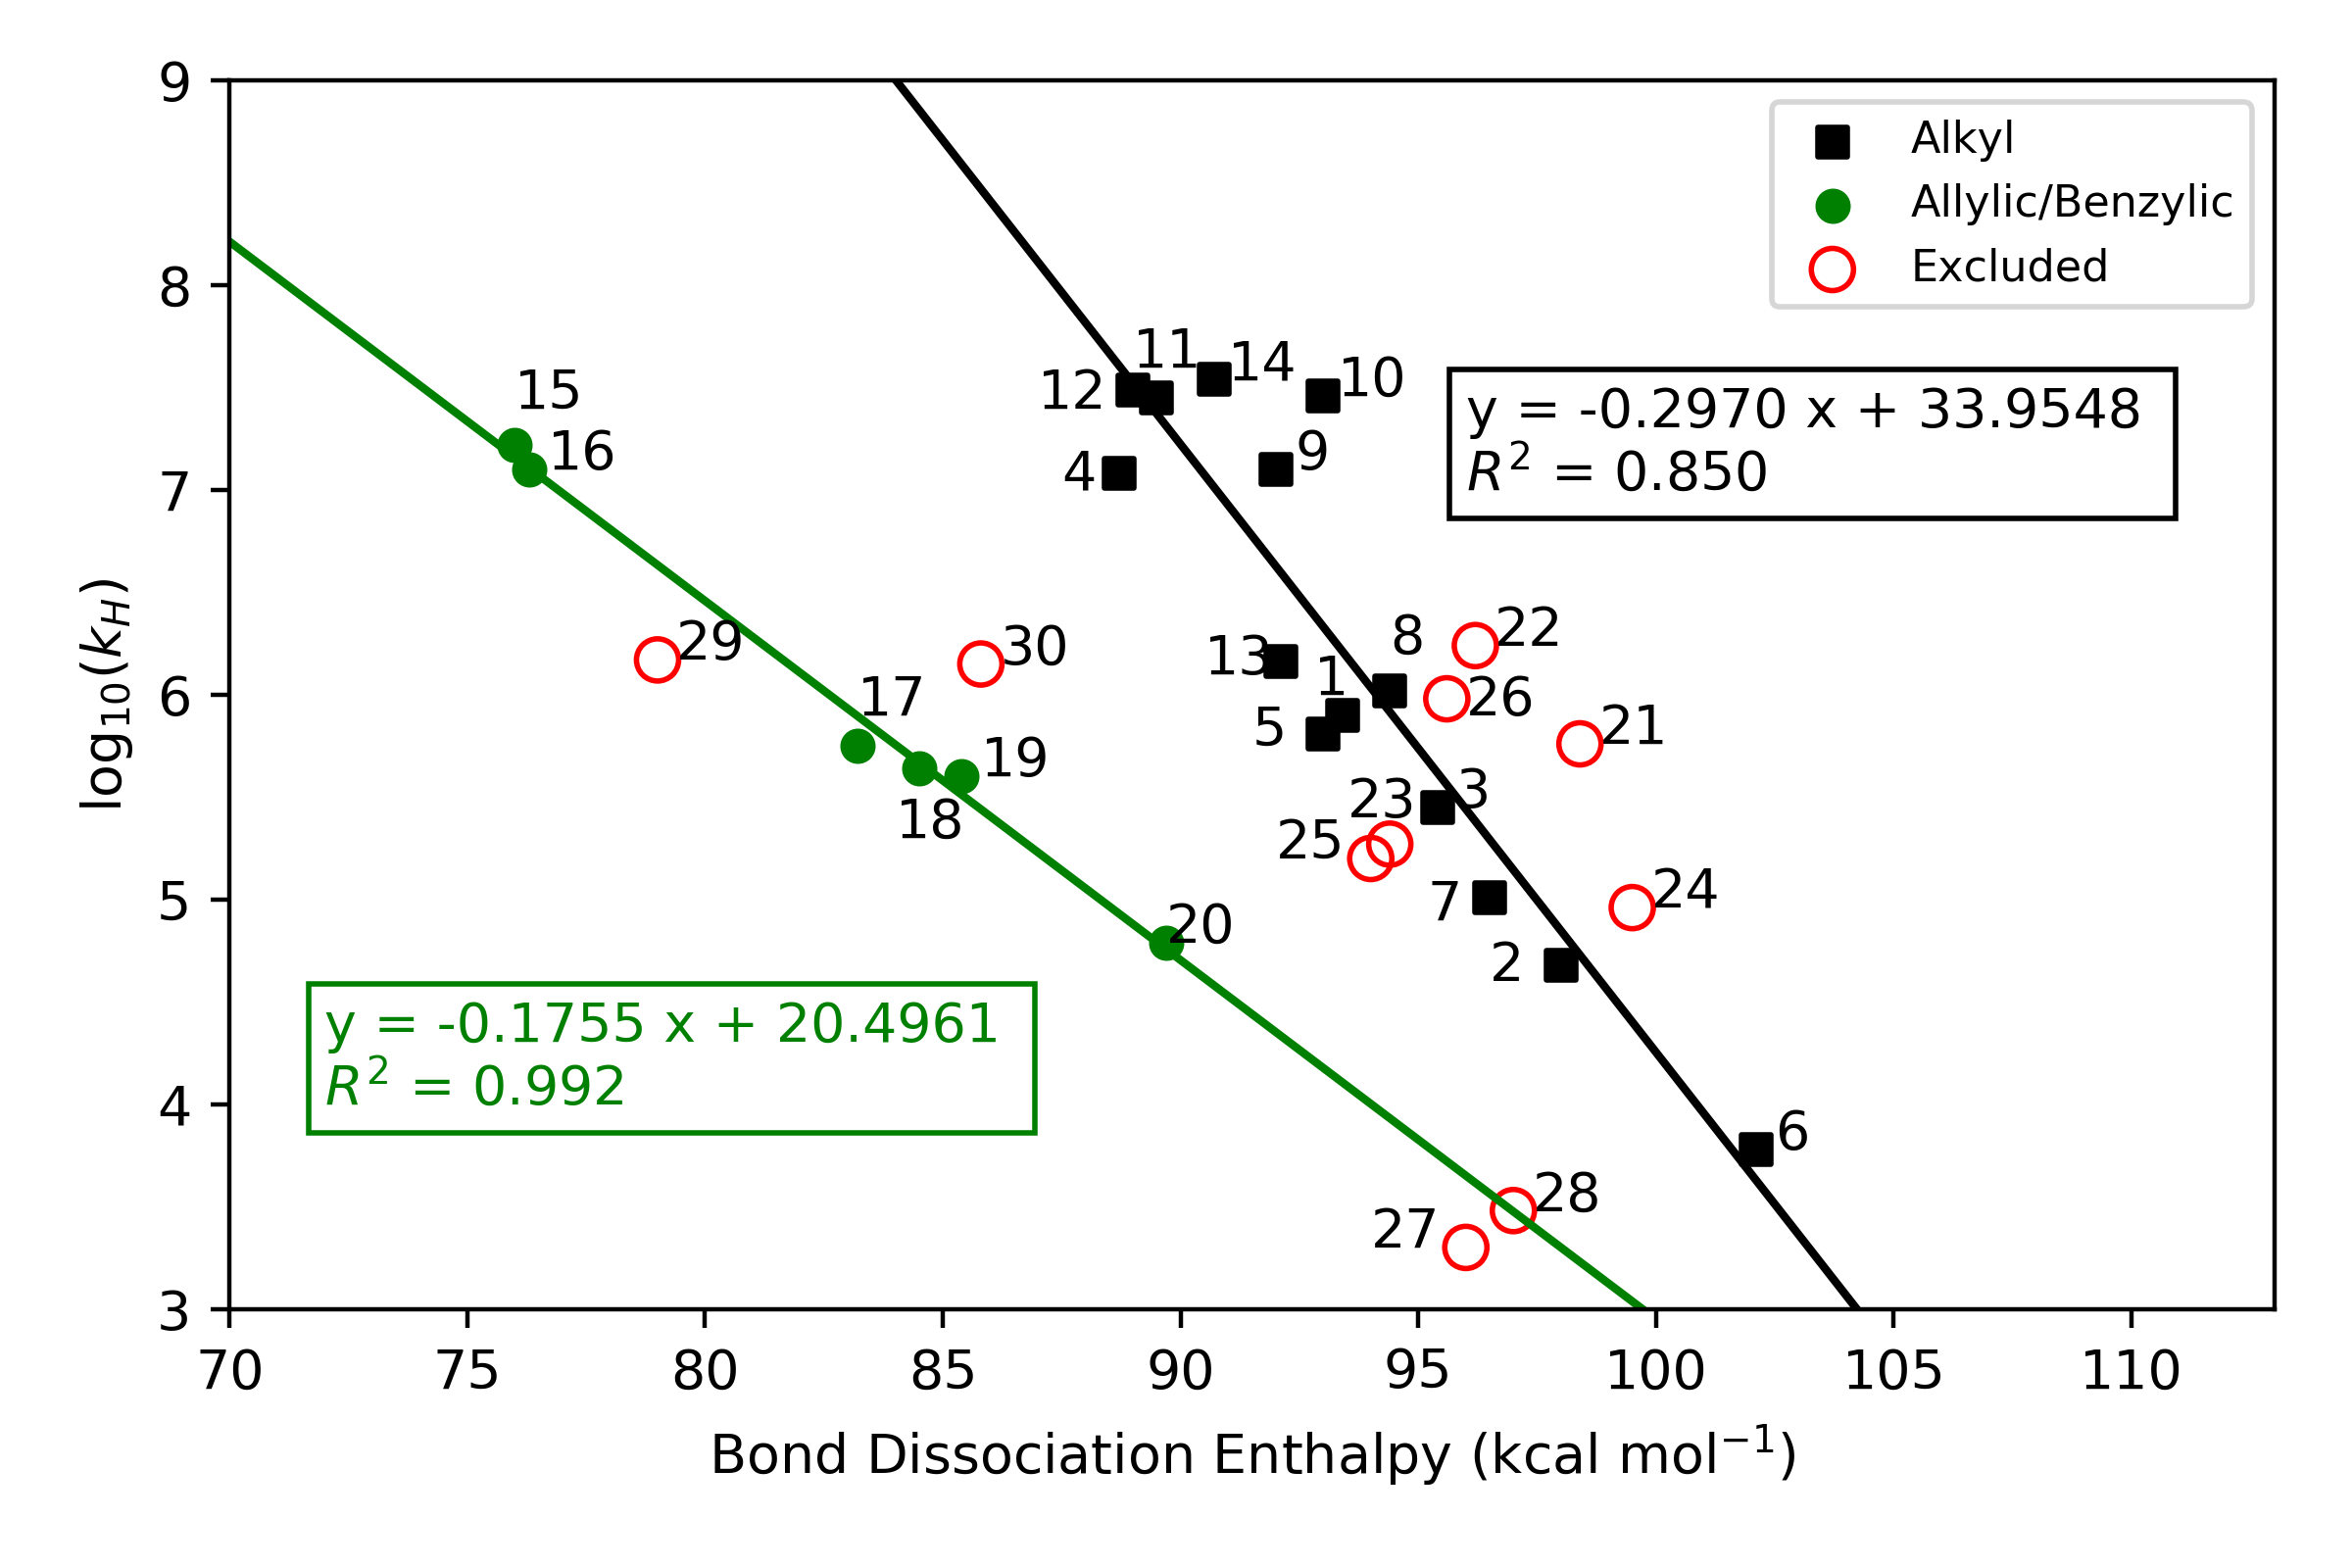
\includegraphics[width=\textwidth]{figures/bep-expt}
\begin{tabularx}{\textwidth}{| l X l X |}
  \hline
  1 & 1,4-diazobicyclo[2.2.2]octane & 2 & 2,2-dimethylbutane \\
  3 & 2,2-dimethylbutane & 4 & Benzaldehyde \\
  5 & Diethyl ether & 6 & Dimethyl sulfoxide \\
  7 & Dioxane & 8 & Hexamethylphosphoramide \\
  9 & Morpholine & 10 & Piperazine \\
  11 & Piperidine & 12 & Pyrroldiine \\
  13 & Tetrahydrofuran & 14 & Triethylamine \\
  15 & 1,4-cyclohexadiene & 16 & 9,10-dihydroanthracene \\
  17 & Cumene & 18 & Diphenylmethane \\
  19 & Ethylbenzen & 20 & Toluene \\
  21 & Adamantane (2$^\circ$) & 22 & Adamantane (3$^\circ$) \\
  23 & Cycloheptane & 24 & Cyclohexane \\
  25 & Cyclooctane & 26 & Cyclopentane  \\
  27 & Acetone & 28 & Acetonitrile \\
  29 & Benzyl alcohol & 30 & Dibenzyl ether \\
  \hline
\end{tabularx}
  \caption[Bell-Evans-Polanyi plot of experimental rate constants against
  literature BDEs.]{Bell-Evans-Polanyi plot of experimental rate constants
  (normalized for the number of equivalent hydrogen atoms) for HAT between
  \cumo\ and substrates against literature BDEs. BDEs for dimethyl sulfoxide
  and hexamethylphosphoramide are from Ref.~\protect\citenum{Salamone2012},
  while all other BDEs are from Ref.~\protect\citenum{Luo2002}. Points 21--26
  and 29--30 were excluded from linear regression as possible outliers.}
  \label{fig:bep-expt}
\end{figure}

There is a considerable amount of scatter in~\ref{fig:bep-expt}, thus possible
outlier were excluded from the initial linear-regression analysis. The scatter
may be due to differences in experimental procedures in the measurement of
BDEs, which are measurable using a large number of different experimental
techniques. A great deal of data exists in the literature, much of which has
conveniently been compiled in the \emph{de facto} reference for BDEs: the
\emph{CRC Handbook of Bond Dissociation Enthalpies}.\cite{Luo2002} However,
caution must be taken with experimentally determined BDEs, as not all
experimental methods give reliable data. For example, BDEs from the
Bordwell\cite{Bordwell1988} thermochemical cycle are possibly
unreliable.\cite{Salamone2012, Miller2016} This was demonstrated for the BDE of
dimethyl sulfoxide (DMSO), for which the experimentally determined BDE is about
8 \kcalmol\ lower than the best computational estimate.\cite{Salamone2012}
Therefore, quantum chemistry is a useful tool for studying BDEs, as it is
relatively simple to compute BDEs. The BDE for an arbitrary \ch{X-H} bond is
given by:

\begin{equation}
  \Delta H(BDE) =  H(\ch{X^.}) + H(\ch{H^.}) - H(\ch{X-H})
\end{equation}

\noindent where $\Delta H(BDE)$ is the BDE, and the right-hand terms are the
enthalpies of the radical product, the hydrogen atom, and the substrate,
respectively. By computing the most accurate BDEs possible, we are able to
discern if the BEP principle holds for \ch{C-H} bond hydrogen abstraction by
\cumo.

Many DFT-based methods have been shown to give reasonably reliable relative
BDEs, that is, the difference in BDE from a reference molecule (often
\ch{CH4}).\cite{DiLabio1999, Chan2012, Wiberg2014} However, highly correlated
wave function based methods are required to predict chemically accurate
(sub-\kcalmol) BDEs. For this purpose, we shall use composite quantum chemical
procedures. Unfortunately, due to the computational cost of some of these
procedures, calculations are often limited to small molecules. For instance,
\citet{Chan2012} recently published a diverse set of high-level BDEs for small
molecules with at most 5 heavy (non-hydrogen) atoms. There is a lack of
literature that compares the ability of common composite methods to predict
accurate \ch{C-H} BDEs for relatively large molecules. Therefore, another aim
of the work is to determine which composite procedure can be used to calculate
accurate BDEs for relatively large molecules.

\section{Methods}\label{sec:hat-methods}

Experimental rate constants were either provided from unpublished results from
our colleagues in Rome, or come from literature sources.\cite{Bietti2010,
Bietti2011, Pischel2001, Salamone2011, Salamone2012, Salamone2012a,
Salamone2013, Salamone2015} All rate constants come from laser flash photolysis
(LFP) experiments of \cumo\ with the substrates of interest. Nitrogen or argon
saturated acetonitrile solvent and ambient conditions (298 K and 1 atm) were
used in all cases. For those results that are unpublished, \cumo\ is generated
by laser pulses at either 266 nm or 355 nm in solutions of excess dicumyl
peroxide. Many of the literature results are also from the Bietti group, where
the same procedure is used. Other results may have small variations in
experimental details, however, all results are well time-resolved.

Observed rate constants ($k_{obs}$) are generally obtained from 2--8 averaged
trials, which are reproducible to within 5\%. Transient absorption decay traces
of \cumo\ monitored at 485 nm are used to determine $k_{obs}$. The observed
rate constant is plotted against concentration of substrate to provide the
bimolecular HAT rate constant ($k_H$) as the slope ($k_{obs} = k_0 +
k_H[substrate]$). The \cumo\ radical decays unimolecularly through the
$\beta$-scission of a methyl group, giving acetophenone and a methyl radical,
as shown in~\ref{fig:cumo-decay}. The unimolecular decay rate
constant\cite{Avila1993, Avila1995} for \cumo\ ($k_0$) in acetonitrile is on
the order of 6.3 \E{5} s$^{-1}$ at 298 K.

\begin{scheme}[H]
  \centering
  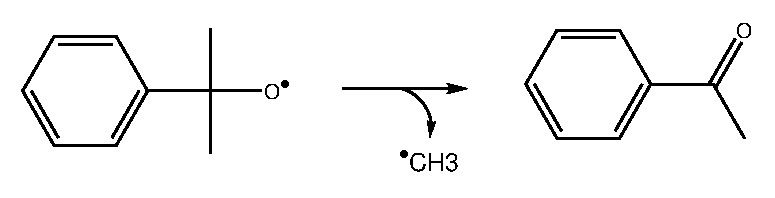
\includegraphics[width=0.75\textwidth]{figures/cumobeta.eps}
\caption{Unimolecular decay of the cumyloxyl radical.}
\label{fig:cumo-decay}
\end{scheme}

All quantum chemical calculations were performed using the Gaussian 09 software
package.\cite{Frisch2009} Several composite quantum chemical methods that are
implemented in Gaussian 09 were used in this work: W1BD, CBS-QB3 and the
restricted open-shell variant ROCBS-QB3, CBS-APNO, G4 and the MP2 variant
G4(MP2). An approach using ROCCSD(T) with locally-dense basis
sets\cite{DiLabio1999LDBS, Wright2001} (LDBS) was also utilized in order to
approximate W1BD results. Each of these methods is briefly described below.


\subsection{Quantum chemical composite procedures}

\noindent \textbf{W1BD}

The highest-accuracy method used is W1BD, which employs seven different
calculations to obtain highly-correlated electronic energies, as well as
thermochemically corrected quantities. This method is very computationally
expensive, and thus cannot be applied to the larger species of interest in this
work. Geometries and thermochemical corrections come from DFT-based B3LYP
calculations with nearly complete cc-pVTZ+d basis sets. A frequency scaling
factor of 0.985 is used to obtain thermochemical corrections. The electronic
energy comes from several additive corrections involving the Brueckner
Doubles\cite{Barnes2009} (BD) variation of coupled cluster and large basis sets
extrapolated to the complete basis set limit. Corrections for core-electron
correlation and relativistic contributions are computed using an uncontracted
variant of the cc-pVTZ+2df basis sets, known as MTsmall.\cite{Martin1999} \\

\noindent \textbf{LDBS approach}

Locally-dense basis sets have been used in the past to calculated BDEs for
relatively large molecules.\cite{DiLabio1998, DiLabio1999LDBS, Wright2001} The
principle behind LDBS is to use large basis sets to treat the atomic centres
that are directly involved in the chemistry taking place, and use progressively
smaller basis sets for ``remote'' portions of the molecule, thus taking
advantage of error cancellation. We chose a method that best approximates W1BD
results for a small subset of molecules. The scheme utilized herein involves
geometry optimization and scaled frequency calculations from DFT-based
B3LYP/cc-pVTZ+d, as used in the W1BD procedure. Single-point energy
calculations are then performed using ROCCSD(T) and an LDBS partitioning scheme
we denote as pc-3/3/2/1, demonstrated in~\ref{fig:ldbs}, using the polarization
consistent basis sets.\cite{Jensen2001}

\begin{scheme}[H]
\centering
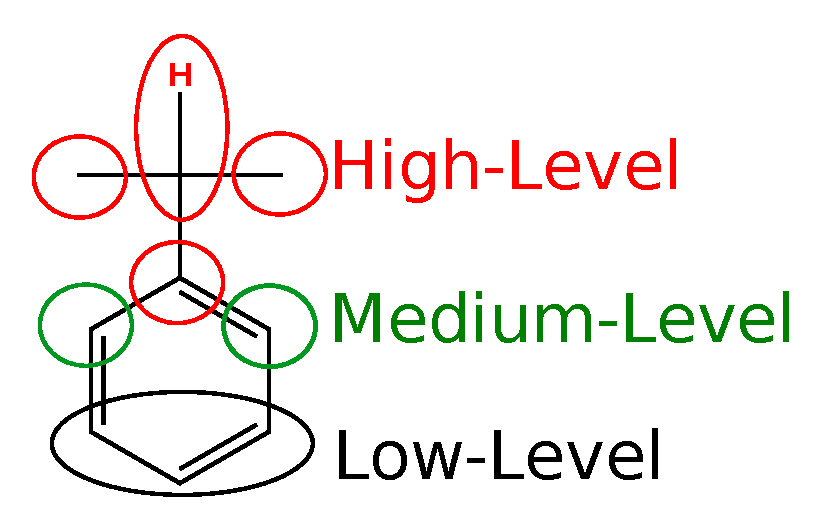
\includegraphics[width=\textwidth]{figures/ldbs.eps}
\caption[Locally-dense basis set partitioning used in the calculation of
BDEs.]{Locally-dense basis set partitioning used in the calculation of BDEs.
The scheme is referred to as pc-3/3/2/1, where for the shown cumene molecule,
the centre of \ch{C-H} cleavage and the immediately adjacent groups are treated
with high-level pc-3 basis sets. The next groups are treated with medium-level
pc-2 basis sets, and all other atoms/groups are treated with low-level pc-1
basis sets.} \label{fig:ldbs}
\end{scheme}

\noindent \textbf{CBS methods}

The Complete Basis Set (CBS) methods of Petersson and
colleagues\cite{Montgomery1999, Montgomery2000, Ochterski1996, Wood2006} are
widely used because of the relatively low computational cost (compared to other
composite procedures), and well-established accuracy.\cite{Somers2015,
Simmie2015} CBS-QB3\cite{Montgomery1999, Montgomery2000} utilizes DFT-based
B3LYP optimization and scaled frequencies (factor = 0.990) with modified
triple-zeta Pople style basis sets. Electronic energies are obtained by
extrapolating medium basis set CCSD(T) and MP4SDQ single point energy
calculations to the complete basis set limit. Small empirical corrections are
added to achieve more accurate results compared to the parametrization
sets.\cite{Petersson2001} ROCBS-QB3 is a similar procedure to CBS-QB3, except
spin-restricted wave functions are used in place of unrestricted wave
functions. This is done to eliminate spin contamination, and the use of a
restricted open-shell definition has been shown to produce more accurate
BDEs.\cite{DiLabio1999} The (RO)CBS-QB3 methods have been implemented for the
first, second, and third periods of elements.

Atomic pair natural orbital (APNO) expansions are a method used for averaging
over multiple Slater determinants. The use of APNOs allows for small basis set
extrapolation of higher order correlation energies to converge more rapidly to
the complete basis set limit. This approach is used in the CBS-APNO
method.\cite{Ochterski1996} Geometries and scaled frequencies (factor = 0.989)
are obtained at the QCISD/6-311G(d,p) level of theory. Similar to CBS-QB3,
extrapolating moderate basis set MP4SDQ and QCISD(T) results gives the
electronic energy. An empirical correction is also used in CBS-APNO. Although
CBS-APNO is more accurate, the expansion of APNOs makes CBS-APNO more
computationally demanding than CBS-QB3. As a result, CBS-APNO has only been
implemented for first and second row periods and thus less commonly used in the
literature.  \\

\noindent \textbf{G$n$ methods}

The Gaussian$-n$ (G$n$) series of methods originates from the Pople
group,\cite{Pople1989} and G4 is the fourth generation. G4 utilizes moderately
large basis sets and extrapolation techniques with CCSD(T) calculations to
obtain highly correlated electronic energies. G4(MP2) uses MP2 in place of
CCSD(T) and is thus less computationally expensive, but also gives a less
complete description of electron correlation. Both methods use the
B3LYP/6-31(2df,p) level of theory for optimization and frequency calculations
with a frequency scaling factor of 0.9854. G4 results have been described as
generally on par with CBS-QB3 results,\cite{Somers2015, Simmie2015} but
calculations are more computationally expensive.

\subsection{Transition state calculations}

Calculations were performed to identify the lowest energy TS complex of several
reactions between \cumo\ and organic substrates. In all cases cisoid and
transoid conformations were explored. All optimization calculations were
performed at the B3LYP-D3(BJ)/6-31+G$^*$ level of theory, followed by
single-point energy calculations at the B3LYP-D3(BJ)/6-311+G(2d,2p) level of
theory with the SMD continuum solvent model\cite{Marenich2009} to approximate
solvent effects. Transition states were visualized using the Chemcraft
program\cite{ccraft} to confirm a single imaginary frequency connecting
reactants to products. In some cases, a small secondary imaginary frequency was
observed, indicating a TS complex that is not fully optimized. Necessary steps
were taken to re-optimize the structures and eliminate the small imaginary
frequencies, however, this was not always successful. Nonetheless, I am
confident the structures reported herein sufficiently represent the true TS
complex geometries and relative energies. Results from structures that are not
fully optimized are indicated appropriately as such.

\section{Comparison of composite method for the prediction of BDEs}

In order to determine the best method for BEP principle analysis, and to
investigate which is the most efficient yet accurate composite method, the BDEs
of 50 species have been calculated. This set of species contains a wide variety
of chemical functionalities with BDEs ranging from 75--113 \kcalmol, thus this
set may be described as a comprehensive test of these methods for C-H BDEs.
Given that W1BD is the most accurate method used, these results have been used
for comparison to other composite methods. However, due to computational cost
restrictions, BDEs for only 33 out of the 50 species studied could be
calculated using W1BD; hard disk capacity was insufficient for large systems.
Therefore, literature BDEs from \citet{Luo2002} for the 49 species that have
literature values in the set are also used for comparison. The literature and
calculated BDEs are listed in~\ref{tab:bde-calc}.

%\singlespacing
\begin{longtable}{m{3.1cm} | c c c c c c c c}
\caption[Bond dissociation enthalpies of the species used to investigate the accuracy of composite methods.]{Bond dissociation enthalpies of the species used to investigate the accuracy of composite methods. All values are in \kcalmol. Statistics are listed at the bottom of the table.} \label{tab:bde-calc} \\
Molecule                         &  Lit.\cite{Luo2002}      &   W1BD   &     LDBS &     CBS-QB3 &   ROCBS-QB3 &   CBS-APNO &    G4   &    G4(MP2)\\
\hline
\endfirsthead
Molecule                         &  Lit.\cite{Luo2002}      &   W1BD   &     LDBS &     CBS-QB3 &   ROCBS-QB3 &   CBS-APNO &    G4   &    G4(MP2)\\
\hline
\endhead
1,3-pentadiene                   &  83.0     &   82.9   &   82.2   &    80.9     &    81.7    &   81.8   &  81.6   &    82.1   \\
1,4-diazabicyclo[2.2.2]-octane   &  93.4     &          &   98.9   &    98.9     &    98.8    &   98.5   &  96.7   &    95.6   \\
1,4-pentadiene                   &  76.6     &   76.2   &   76.0   &    74.2     &    75.0    &   75.2   &  75.1   &    75.7   \\
2,2-dimethylbutane               &  98.0     &   99.3   &   99.1   &    99.4     &    99.3    &   99.7   &  97.5   &    96.7   \\
2,3-dimethylbutane               &  95.4     &   97.8   &   97.7   &    97.9     &    97.8    &   98.0   &  96.2   &    95.5   \\
2-methylbutane                   &  95.8     &   97.3   &   97.2   &    97.3     &    97.1    &   97.3   &  95.9   &    95.5   \\
Acetaldehyde                     &  94.3     &   95.9   &   95.3   &    95.3     &    95.7    &   95.5   &  94.9   &    94.8   \\
Acetone                          &  96.0     &   96.9   &   96.4   &    96.2     &    96.7    &   97.1   &  95.4   &    95.0   \\
Acetonitrile                     &  97.0     &   96.9   &   96.6   &    96.2     &    96.6    &   96.5   &  96.3   &    96.3   \\
Adamantane (2$^\circ$)           &  98.4     &          &  100.9   &   100.5     &   100.4    &  100.9   &  97.8   &    96.3   \\
Adamantane (3$^\circ$)           &  96.2     &          &  100.3   &    99.9     &    99.9    &  100.3   &         &    95.7   \\
Benzaldehyde                     &  88.7     &          &   90.9   &    91.5     &    91.4    &   91.0   &  89.3   &    88.2   \\
Benzene                          & 112.9     &  113.1   &  112.7   &   115.4     &   113.0    &          &         &   113.0   \\
Benzyl Alcohol                   &  79.0     &          &   84.4   &    84.3     &    83.2    &   83.9   &  83.4   &    83.6   \\
Cumene                           &  83.2     &          &   87.9   &    87.9     &    86.9    &          &  86.9   &    86.7   \\
Cycloheptane                     &  94.0     &          &   96.0   &    96.0     &    95.8    &   96.1   &  93.9   &    92.9   \\
Cyclohexadiene                   &  76.0     &   76.3   &   76.2   &    74.3     &    75.0    &          &  75.2   &    75.5   \\
Cyclohexane                      &  99.5     &   99.2   &   99.1   &    99.4     &    99.3    &   99.6   &  97.5   &    96.8   \\
Cyclooctane                      &  94.4     &          &   92.6   &    92.6     &    92.4    &   92.8   &  90.2   &    89.1   \\
Cyclopentane                     &  95.6     &   96.3   &   96.1   &    96.5     &    96.3    &   96.6   &  95.6   &    95.0   \\
Cyclopropane                     & 106.3     &  109.0   &  108.5   &   109.3     &   109.2    &  109.5   & 108.2   &   108.0   \\
Dibenzyl ether                   &  85.8     &          &   83.6   &    84.3     &    82.7    &          &         &    79.6   \\
Diethyl ether                    &  93.0     &   95.3   &   95.1   &    95.6     &    95.5    &   95.4   &  93.8   &    93.1   \\
Dihydroanthracene                &  76.3     &          &   80.4   &    80.9     &    78.1    &          &         &    79.9   \\
Dimethylamine                    &  94.2     &   92.6   &   92.4   &    92.9     &    92.8    &   92.7   &  92.0   &    91.9   \\
Dimethylsulfoxide                &  94.0     &  102.0   &  101.7   &   102.3     &   102.3    &          & 100.9   &   100.6   \\
Dioxane                          &  96.5     &   97.3   &   97.3   &    97.7     &    97.6    &   97.4   &  95.7   &    94.9   \\
Diphenylmethane                  &  84.5     &          &   84.1   &    85.3     &    82.8    &          &         &    84.5   \\
Ethane                           & 100.5     &  101.3   &   99.3   &   101.7     &   101.5    &  101.8   & 100.7   &   100.7   \\
Ethylbenzene                     &  85.4     &          &   88.3   &    88.6     &    87.6    &   89.3   &  87.6   &    87.7   \\
Ethylene                         & 110.9     &  110.8   &  110.3   &   110.6     &   110.9    &  111.1   & 109.9   &   110.2   \\
Fluorene                         &  82.0     &          &   82.4   &    83.6     &    81.9    &          &         &    81.2   \\
Formaldehyde                     &  88.0     &   88.6   &   88.0   &    89.1     &    88.9    &   88.2   &  88.2   &    87.9   \\
Hexamethyl-phosphoramide         &           &          &   93.8   &    94.1     &    93.9    &          &         &    88.5   \\
Indene                           &  83.0     &          &   80.6   &    80.4     &    80.1    &   81.2   &  79.0   &    78.3   \\
Methane                          & 105.0     &  105.0   &  104.4   &   105.4     &   105.2    &  105.4   & 104.5   &   104.6   \\
Methanol                         &  96.1     &   96.4   &   96.0   &    96.9     &    96.8    &   96.6   &  96.0   &    95.8   \\
Methylamine                      &  93.9     &   93.1   &   92.8   &    93.4     &    93.3    &   93.3   &  92.7   &    92.8   \\
Morpholine                       &  92.0     &          &   93.4   &    93.4     &    93.3    &   93.3   &  91.8   &    91.1   \\
N,N-dimethylacetamide (acetyl)   &  91.4     &   99.6   &   99.4   &    99.5     &    99.5    &  100.1   &  97.6   &    96.8   \\
Piperazine                       &  93.0     &   93.4   &   93.5   &    93.6     &    93.5    &   93.4   &  91.9   &    91.2   \\
Piperidine                       &  89.5     &   92.1   &   92.2   &    92.3     &    92.2    &   92.1   &  90.7   &    90.0   \\
Propane                          & 100.9     &  101.6   &  101.3   &   102.0     &   101.8    &  102.1   & 100.7   &   100.4   \\
Pyrrolidine                      &  89.0     &   90.8   &   90.6   &    90.8     &    90.7    &   90.7   &  89.5   &    89.0   \\
Tetrahydro-2H-pyran              &  96.0     &   96.3   &   96.2   &    96.6     &    96.5    &   96.3   &  94.7   &    93.9   \\
Tetrahydrofuran                  &  92.1     &   93.7   &   93.3   &    93.9     &    93.8    &   93.6   &  92.2   &    91.6   \\
Toluene                          &  89.7     &   90.5   &   90.1   &    90.6     &    89.7    &   91.9   &  89.8   &    90.2   \\
Trichloromethane                 &  93.8     &   93.5   &   93.4   &    93.8     &    93.7    &          &  92.4   &    92.0   \\
Triethylamine                    &  90.7     &          &   91.4   &    91.3     &    91.2    &   91.4   &  89.4   &    88.4   \\
Trifluormethane                  & 106.4     &  107.2   &  106.6   &   107.4     &   107.4    &  106.8   & 105.8   &   105.0   \\
\hline
\textbf{Statistics}             & Lit.       &  W1BD    &    LDBS  &    CBS-QB3  &  ROCBS-QB3  &  CBS-APNO &    G4  &    G4(MP2)\\
\hline
Number of BDEs ($N$) &    49     &     33   &     50   &      50     &      50     &     40    &    43   &     50   \\
MAE (Lit.)                       &           &   0.82   &   1.60   &    1.88     &    1.64     &   1.35    &  1.21   &   1.57   \\
Max. Error                             &           &   1.59   &   2.41   &    2.63     &    3.15     &   1.85    &  4.19   &   6.23   \\
Min. Error                           &           &  -8.22   &  -8.04   &   -8.26     &   -8.25     &  -8.74    & -6.86   &  -6.58   \\
MAE (W1BD)                       &           &          &   0.22   &    0.32     &    0.18     &   0.20    &  0.70   &   0.88   \\
Max. Error                            &           &          &   2.00   &    2.01     &    1.26     &   1.08    &  2.05   &   2.84   \\
Min. Error                            &           &          &  -0.09   &   -2.37     &   -0.35     &  -1.39    &  0.37   &   0.02   \\
\end{longtable}


Mean absolute error (MAE) is used to assess the quality of computational
methods, where errors are calculated with respect to benchmark values for a
given data set.\cite{Savin2014} The MAE is calculated as

\begin{equation}
  \mathrm{MAE} = \frac{1}{N} \sum | E_{ref} - E_{calc}|
\end{equation}

\noindent where, for a set of $N$ reference values, the MAE is the average of
the mean differences of the reference energy ($E_{ref}$) and the calculated
value ($E_{calc}$). The MAE with respect to W1BD and literature shall be
reported herein as ``MAE$_{\mathrm{W1BD}}$ (MAE$_{\mathrm{Lit.}}$)''. An
additional semi-quantitative metric which I used to evaluate the accuracy of
composite procedures to reproduce experimental results is a bar chart that
summarizes the number of deviations from literature within given error ranges.
This bar chart is reported in~\ref{fig:maebarchart}. Note that calculations for
some species with some methods failed to converge, thus number of BDEs out of
49 are also shown in~\ref{fig:maebarchart}. Also, an alternative method that I
shall utilize for reporting these data is through the use of one-to-one plots,
in which BDEs from two methods are directly compared. An ideal plot should have
a slope = 1 and y-intercept = 0.

\begin{figure}[!htbp]
  \centering
  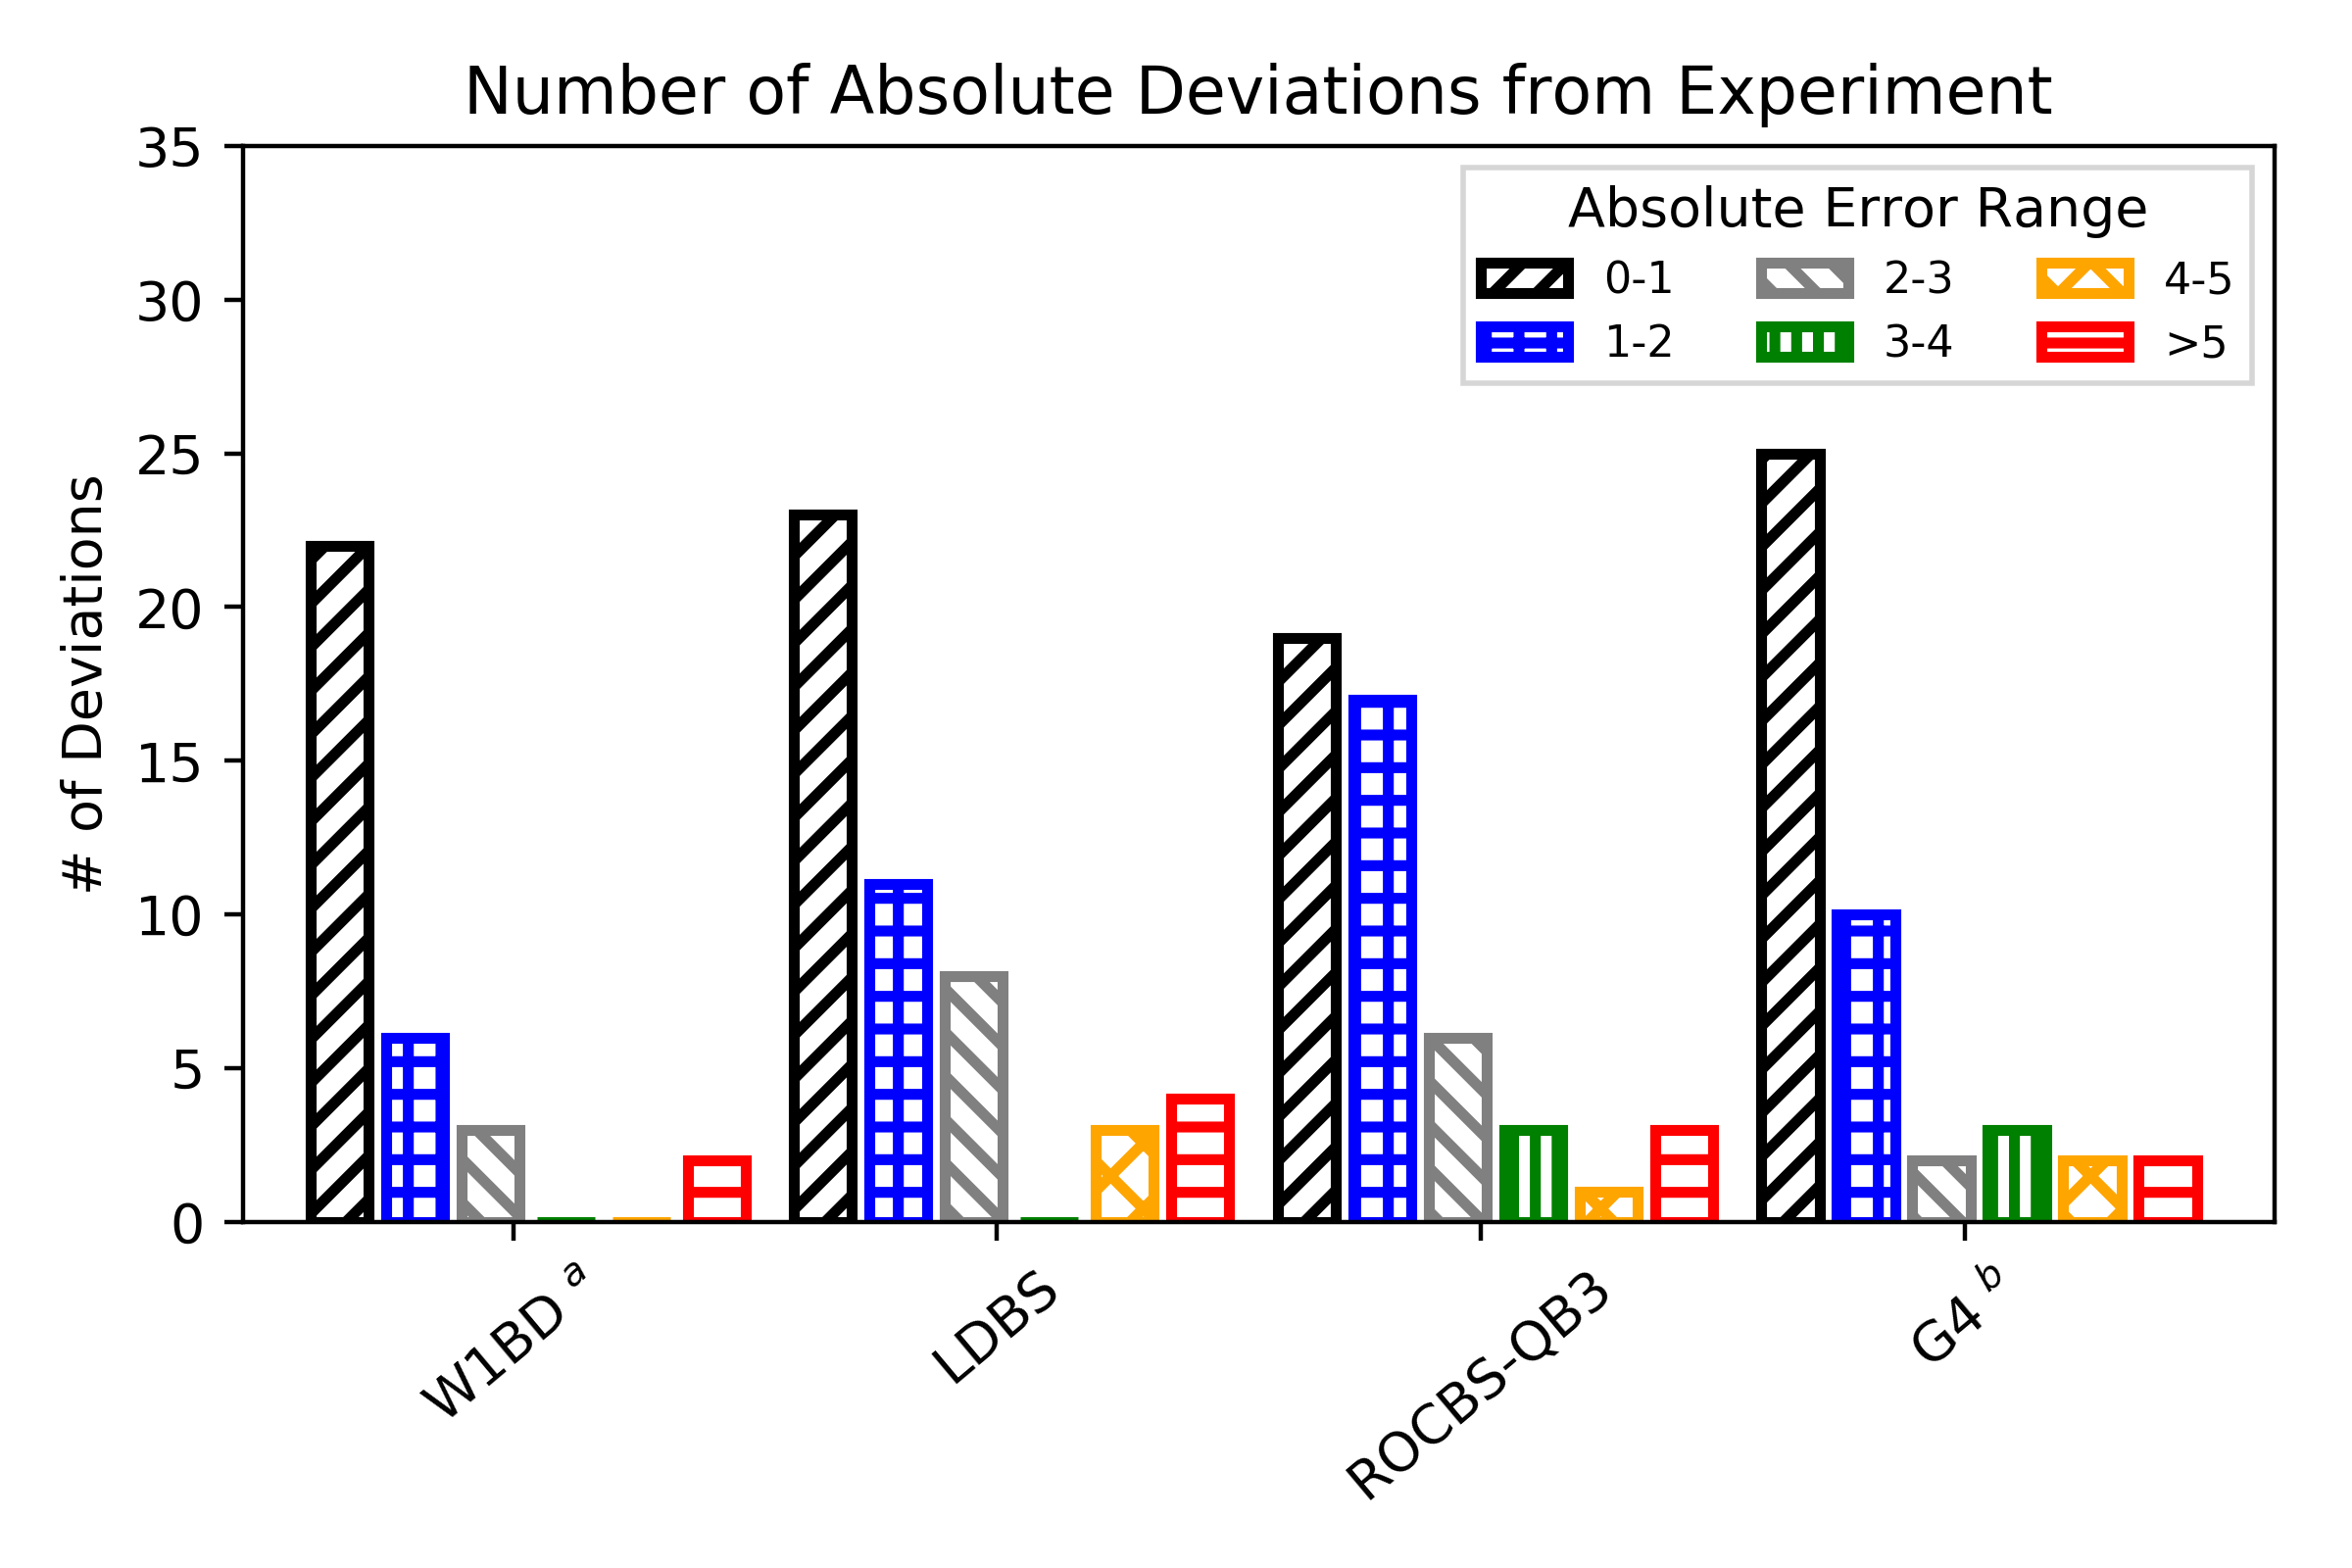
\includegraphics[width=\textwidth]{figures/bde-barchart}
  \caption[Summary of deviations of BDEs from literature for composite quantum
  chemical methods.]{Summary of deviations of BDEs from literature or composite
  quantum chemical methods. Errors are units of \kcalmol\ and are relative to
  Ref.~\protect\citenum{Luo2002}. $^a$ Includes BDEs for 33/49 substrates. $^b$
  Includes BDEs for 40/49 substrates.} \label{fig:maebarchart}
\end{figure}

Comparing W1BD results to literature, the MAE is 0.82 \kcalmol, and the
majority of the data match to within 1--2 \kcalmol of literature. Thus, W1BD is
largely consistent with the literature values. Additionally, the one-to-one
plots comparing W1BD to literature in~\ref{fig:1-1-W1BD} show reasonable
agreement with slope of 0.98 and a y-intercept of 2.35. There are, however, two
notable outliers: DMSO\footnotemark\ and \emph{N,N}-dimethylacetamide, for
which experiment underestimates the BDEs by -8.0 and -8.2 \kcalmol,
respectively. DMSO and \emph{N,N}-dimethylacetamide are consistently outliers
amongst all composite methods, suggesting the literature BDEs are incorrect.

\footnotetext{The experimental BDE for dimethyl sulfoxide was previously
identified as being inaccurate by Salamone et al.\protect\cite{Salamone2012}}

\begin{figure}[H]
  \centering
  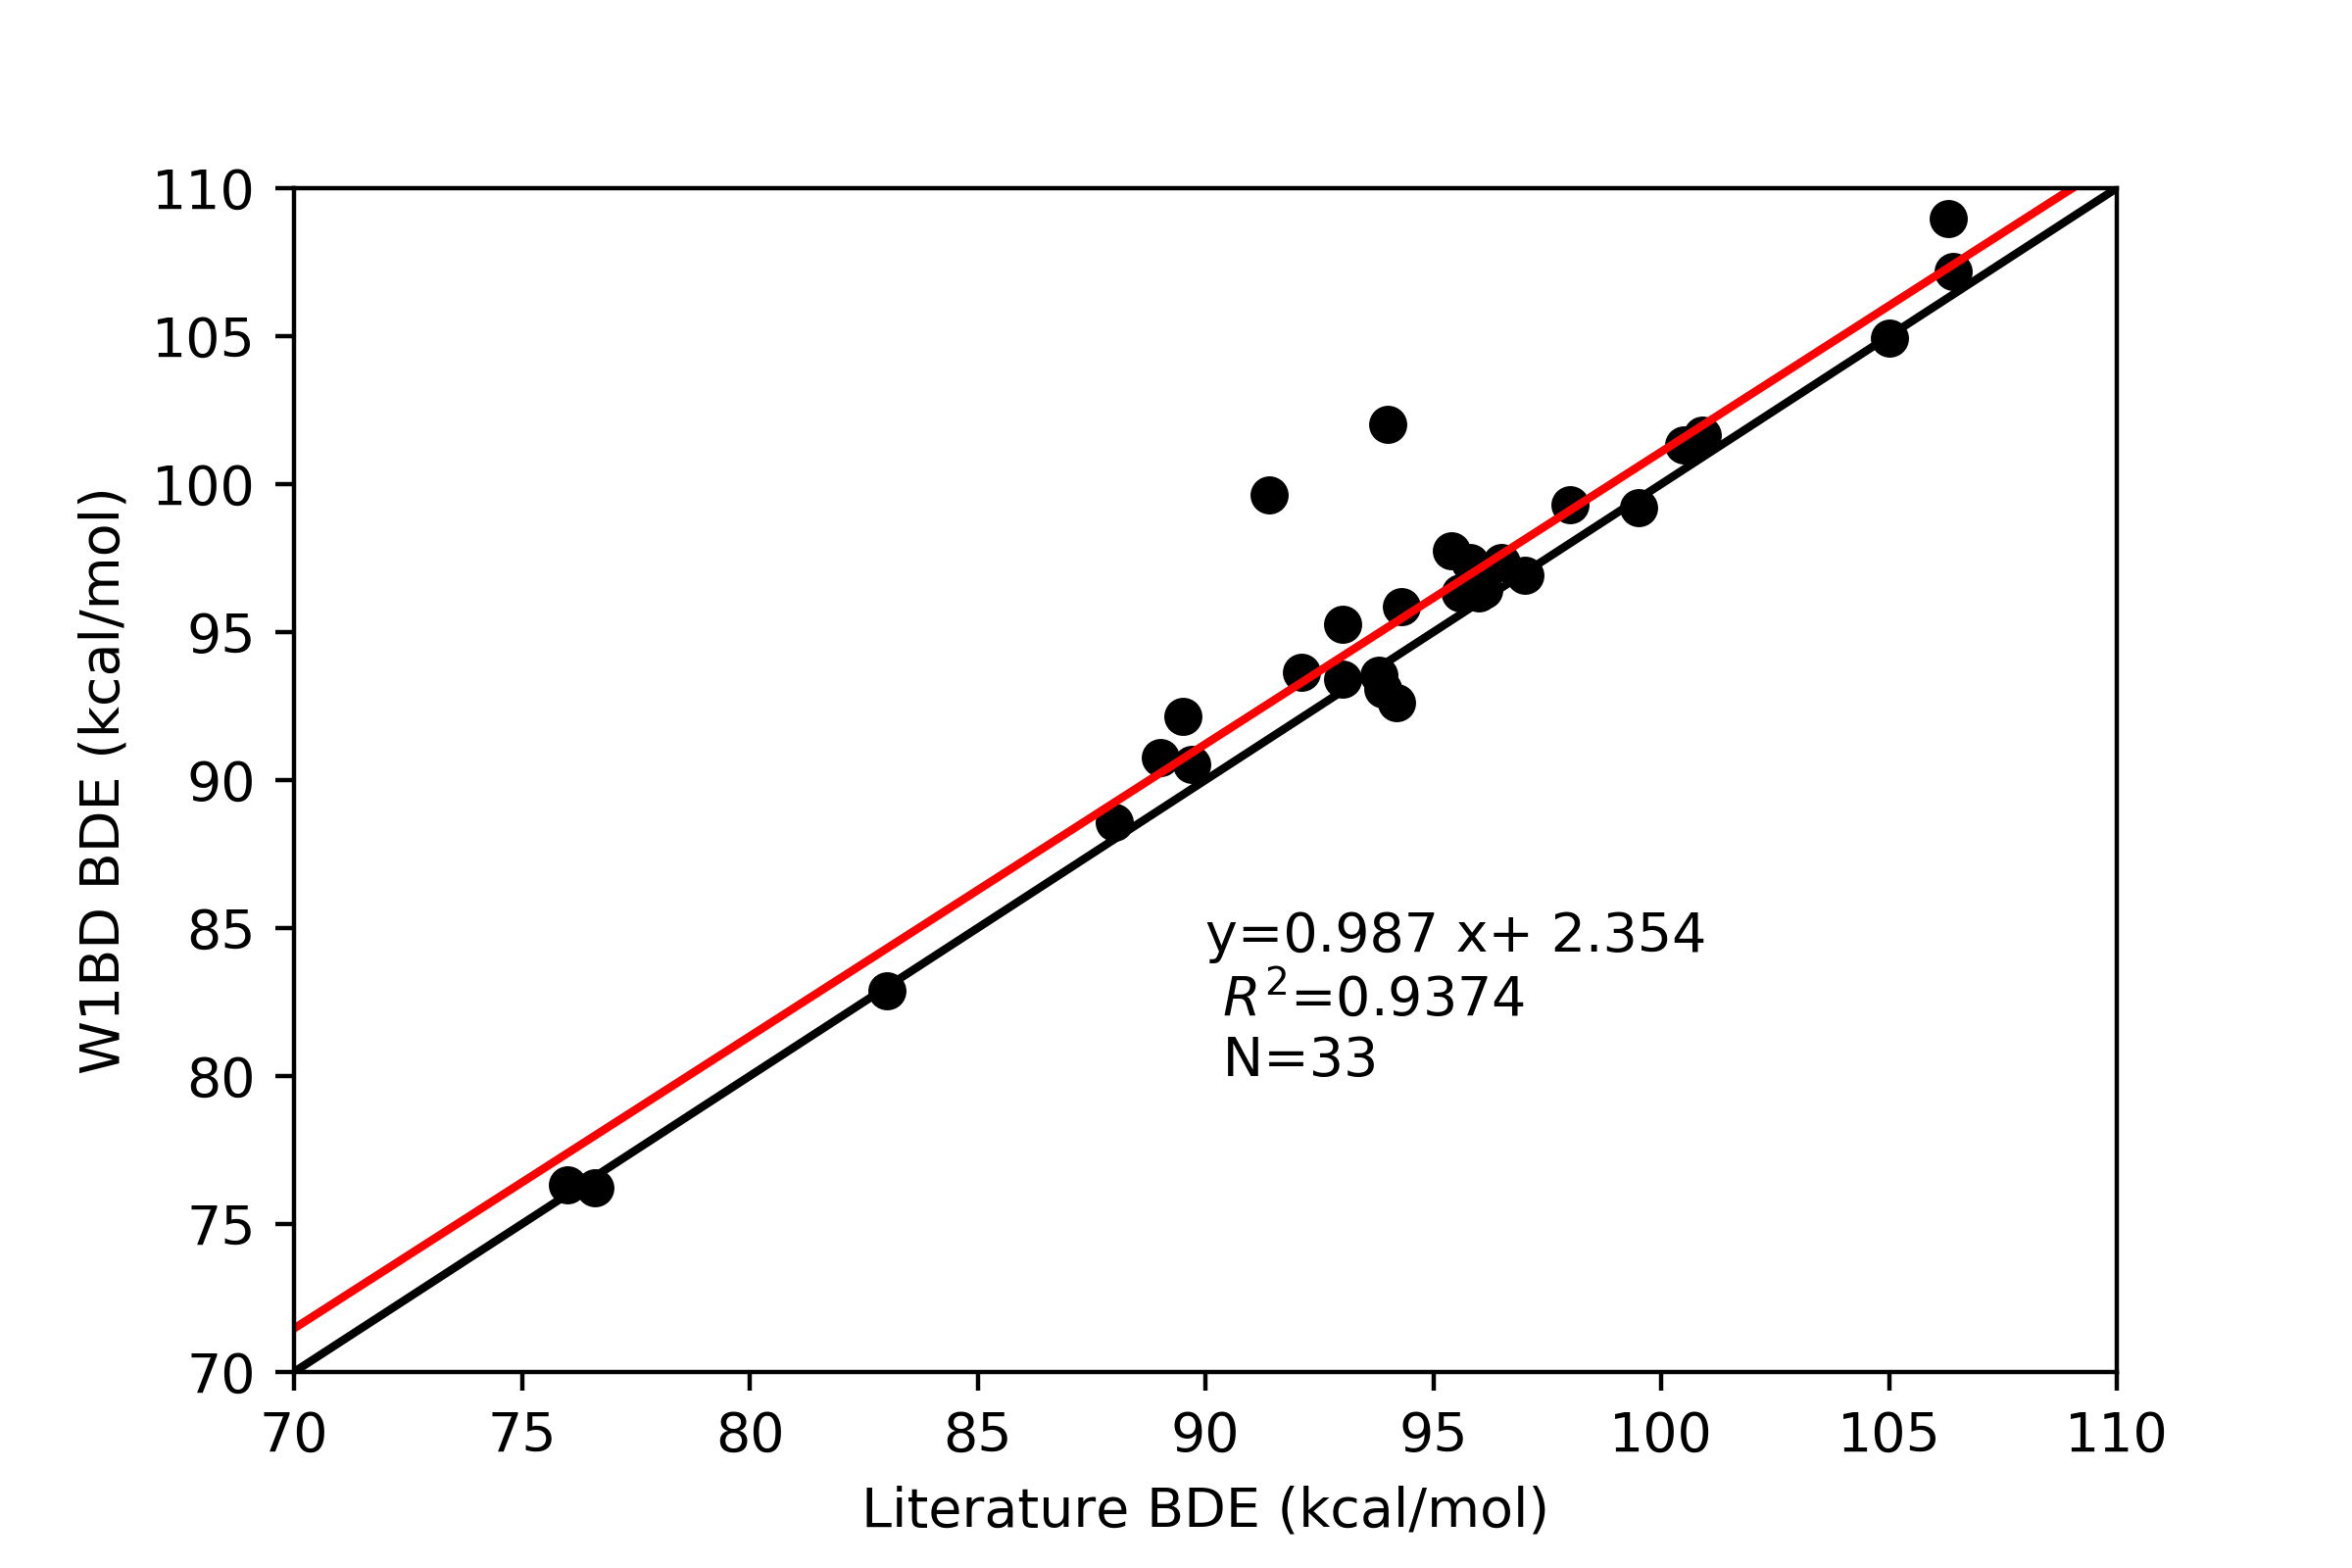
\includegraphics[width=\textwidth]{figures/lit-w1bd}
  \caption[One-to-one plot of BDEs from literature and as calculated by the
  W1BD composite method.]{One-to-one plot of BDEs from
  literature\protect\cite{Luo2002} and as calculated by the W1BD composite
  method. The red dashed-line represents the least squares line of best fit,
  while black line represents a perfect one-to-one correlation.}
  \label{fig:1-1-W1BD}
\end{figure}

The method that gives the best combined agreement with W1BD and literature is
ROCBS-QB3 with an MAE = 0.18 (1.64) \kcalmol. It is also apparent, from the
one-to-one plots in~\ref{fig:1-1-ROCBSQB3}, that ROCBS-QB3 matches well with
literature and experiment. In comparison, CBS-QB3 has an MAE = 0.32 (1.88)
\kcalmol, while CBS-APNO has an MAE = 0.20 (1.40) \kcalmol. The LDBS approach
also performs well with an MAE = 0.22 (1.60) \kcalmol. The G4 method deviates
from the W1BD reference by about 0.5 \kcalmol\ more, however, it appears to
give reasonable agreement with experimental results (MAE = 0.70 (1.21) mol).
The use of the MP2 variant of G4 gives somewhat questionable results, with an
MAE of 0.88 (1.60) \kcalmol, as well as a large outlier of 6.2 \kcalmol\ that
is not present in the other data from composite methods. One-to-one plots of
all other methods are presented in Appendix~\ref{ap:bde}.

\begin{figure}[H]
  \hspace*{-1.5cm}
  \begin{minipage}{8cm}
    \centering
    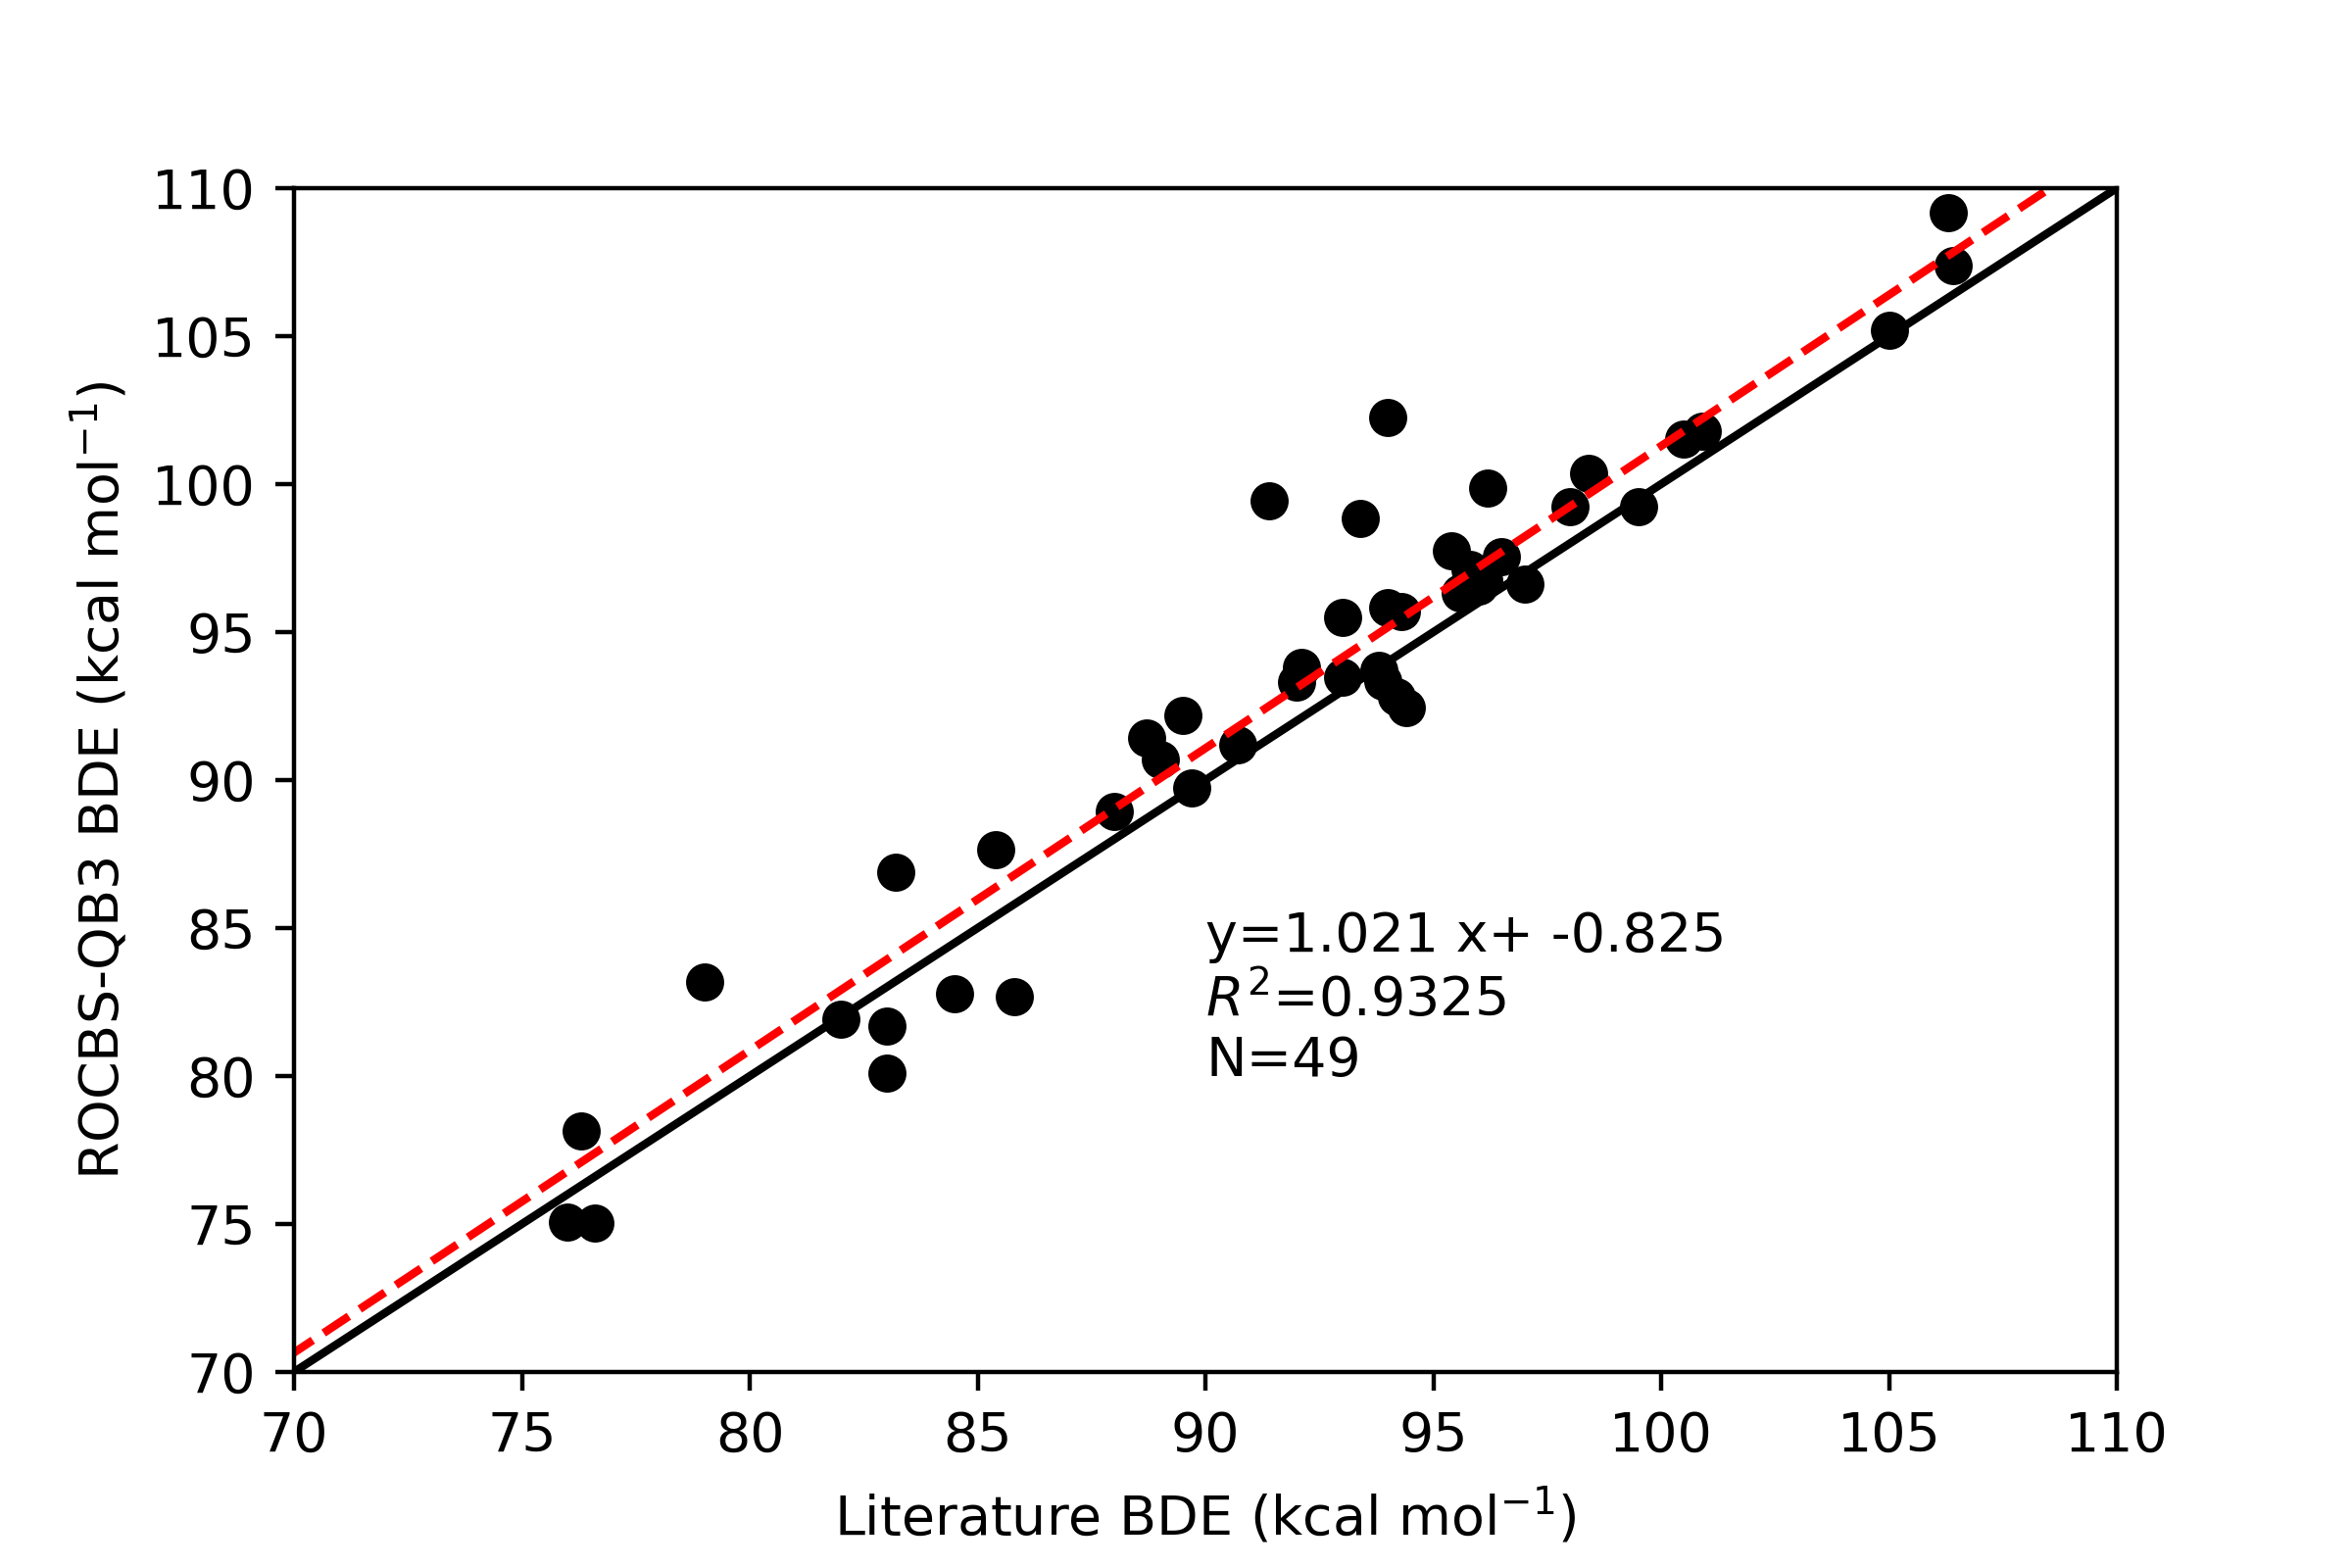
\includegraphics[width=\textwidth]{figures/lit-rocbsqb3}
  \end{minipage}%
  \begin{minipage}{8cm}
    \centering
    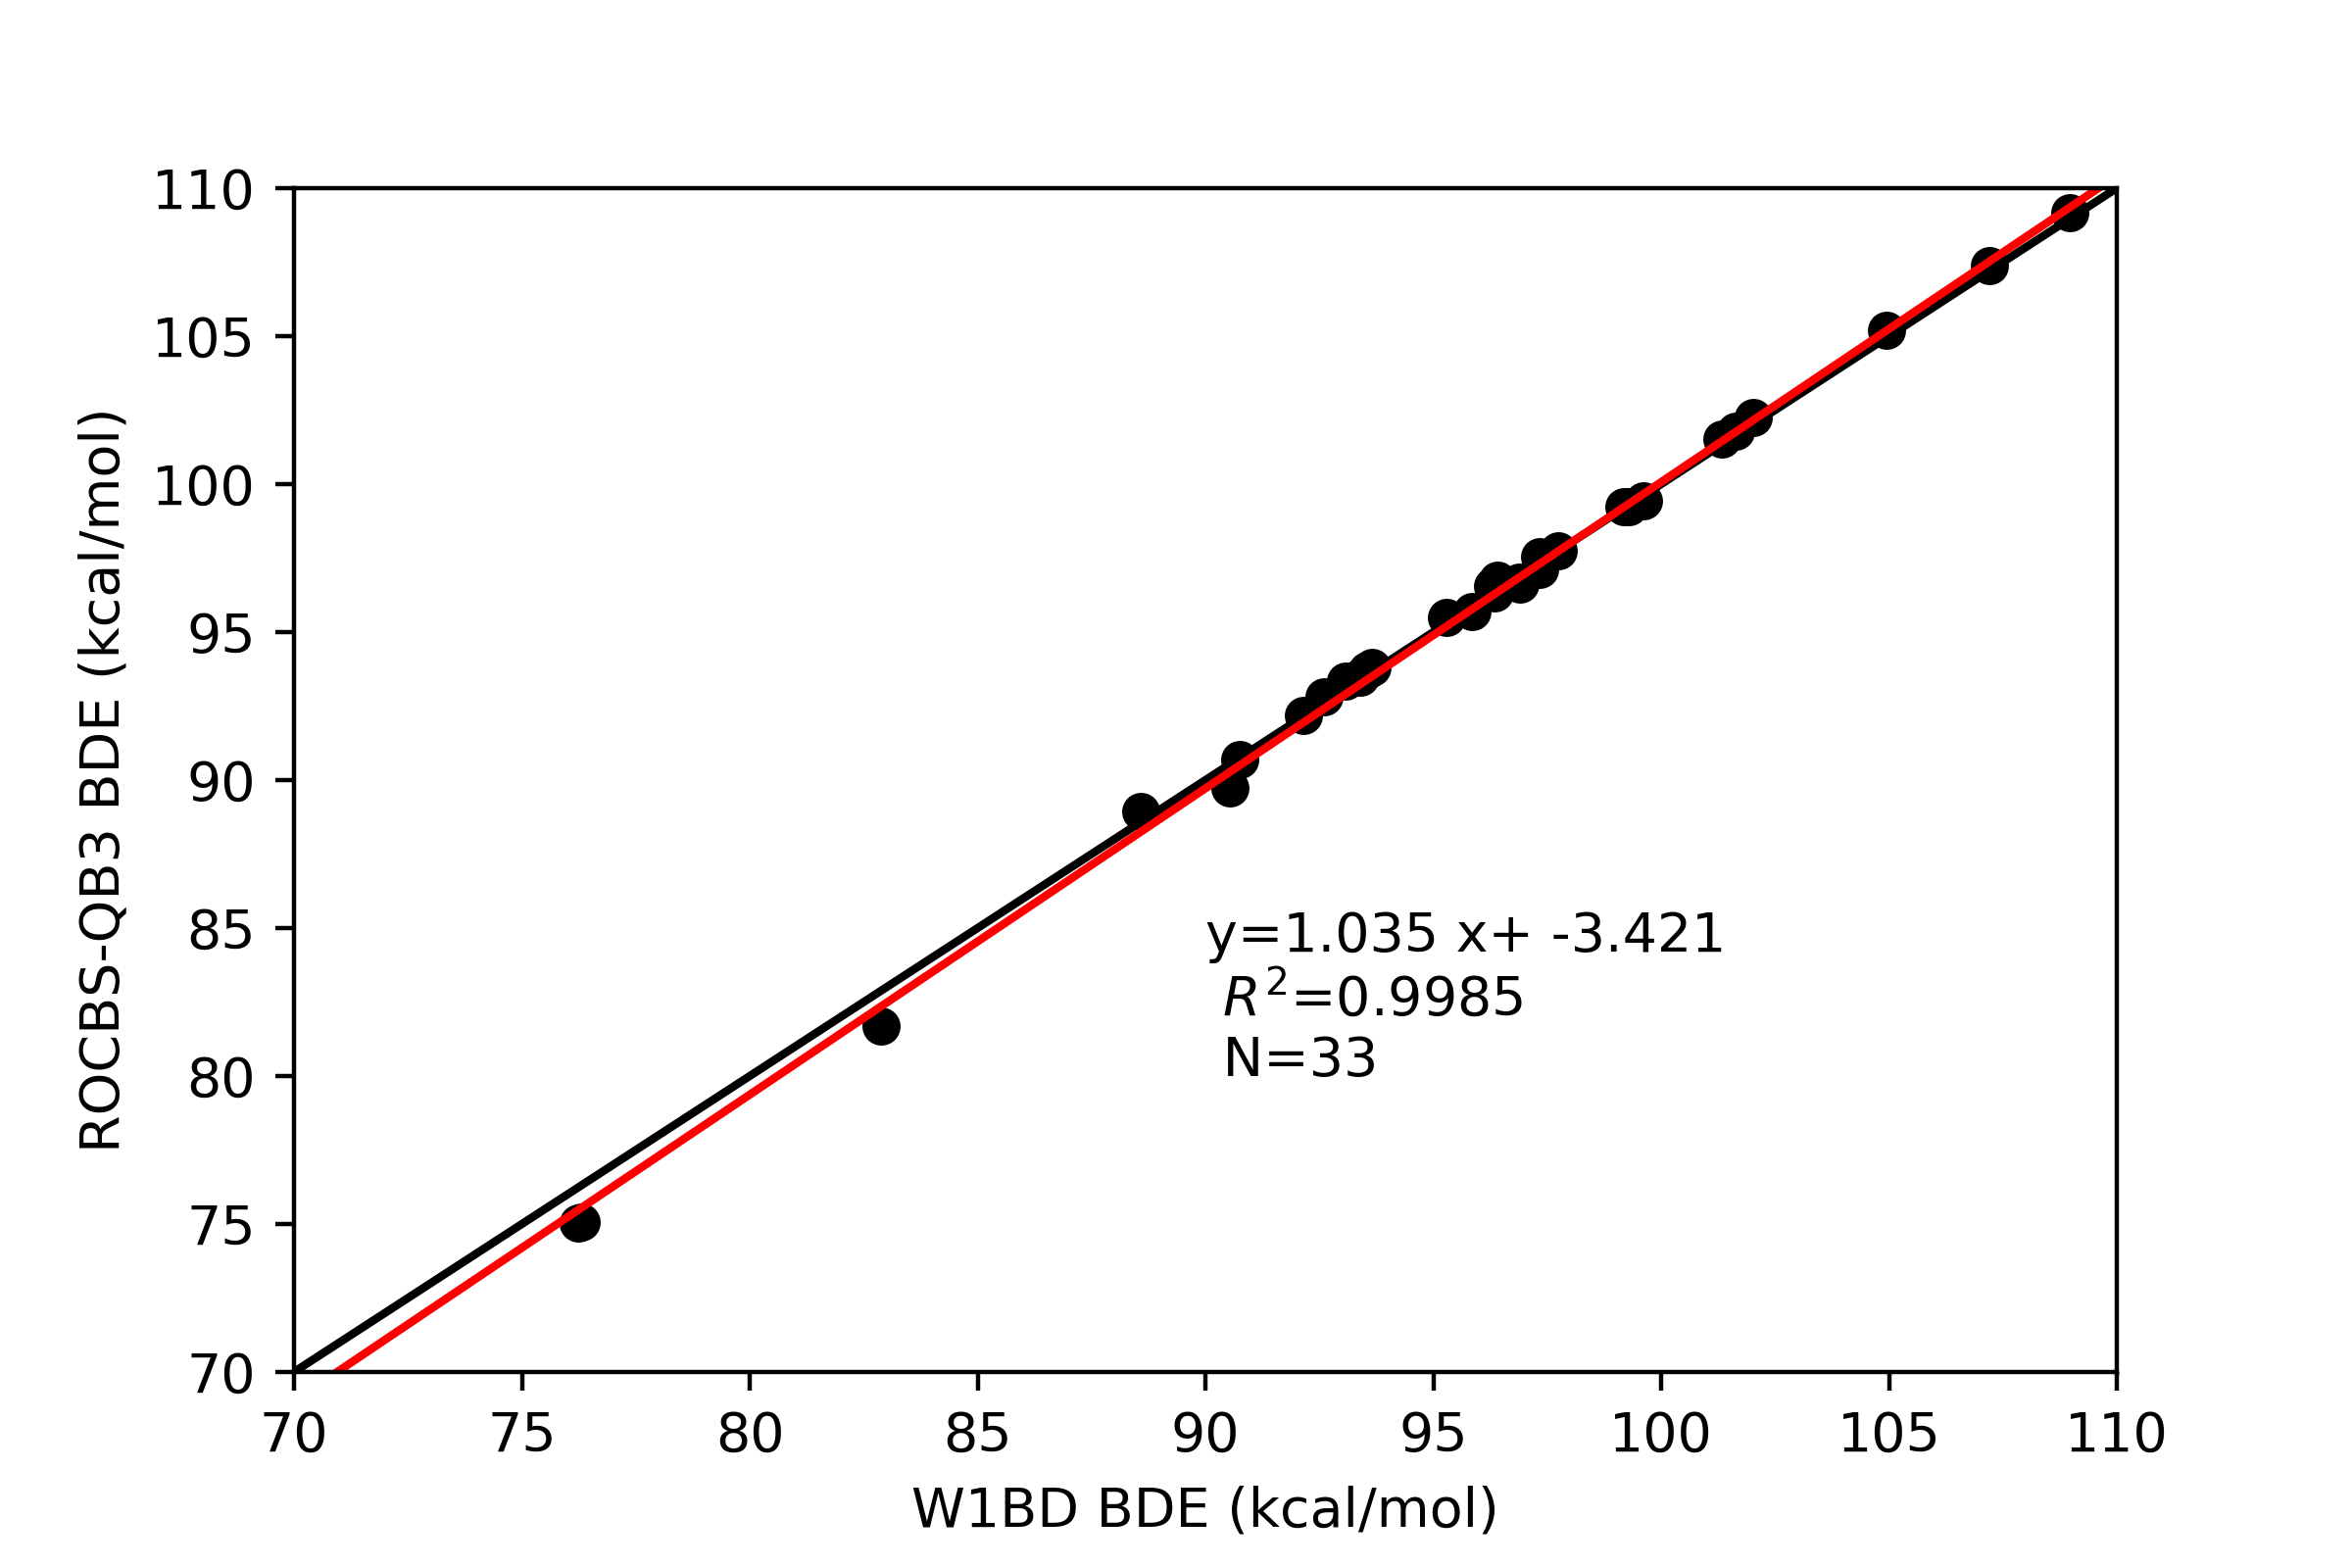
\includegraphics[width=\textwidth]{figures/w1bd-rocbsqb3}
  \end{minipage}
  \caption[One-to-one plot comparing BDEs calculated by ROCBS-QB3 to literature
  and W1BD BDEs.]{One-to-one plot comparing calculated BDEs calculated by the
  ROCBS-QB3 to reference literature\protect\cite{Luo2002} and W1BD BDE values,
  respectively. The red dashed-line represents the least squares line of best
  fit, while black line represents a perfect one-to-one correlation.}
  \label{fig:1-1-ROCBSQB3}
\end{figure}

In summary, ROCBS-QB3 performs best for the calculation of \ch{C-H} BDEs while
G4(MP2) performs worst. Given these data, and considering the relative
computational cost, I recommend the ROCBS-QB3 for the calculation of accurate
BDEs, particularly for large molecules for which more expensive computational
methods are not possible. Importantly, we can now confidently continue
investigating the BEP relationships using reliably calculated BDE data from the
ROCBS-QB3 method. Furthermore, these results can be extended to even larger
systems as the ROCBS-QB3 approach is one of the least computationally-expensive
composite methods. For example, calculations on the cyclohexane molecule, which
take about 20 minutes using ROCBS-QB3 on SGI Altix compute nodes with 6
processors and 8 GB RAM, while G4 takes approximately 27 times longer, the LDBS
approach takes about 500 times longer, and W1BD takes about 1100 times longer.

\section{Analysis of the Bell-Evans-Polanyi principle}

We turn now to the application of accurate BDEs to the BEP principle.
Experimental HAT rate constants have been collected for 32 reactions involving
\cumo\ and organic substrates. The BEP plot of the logarithm of rate constants
divided by the number of equivalent H atoms (i.e., normalized) against BDEs is
shown in~\ref{fig:bde-bep}.

\begin{figure}[!htbp]
  \centering
  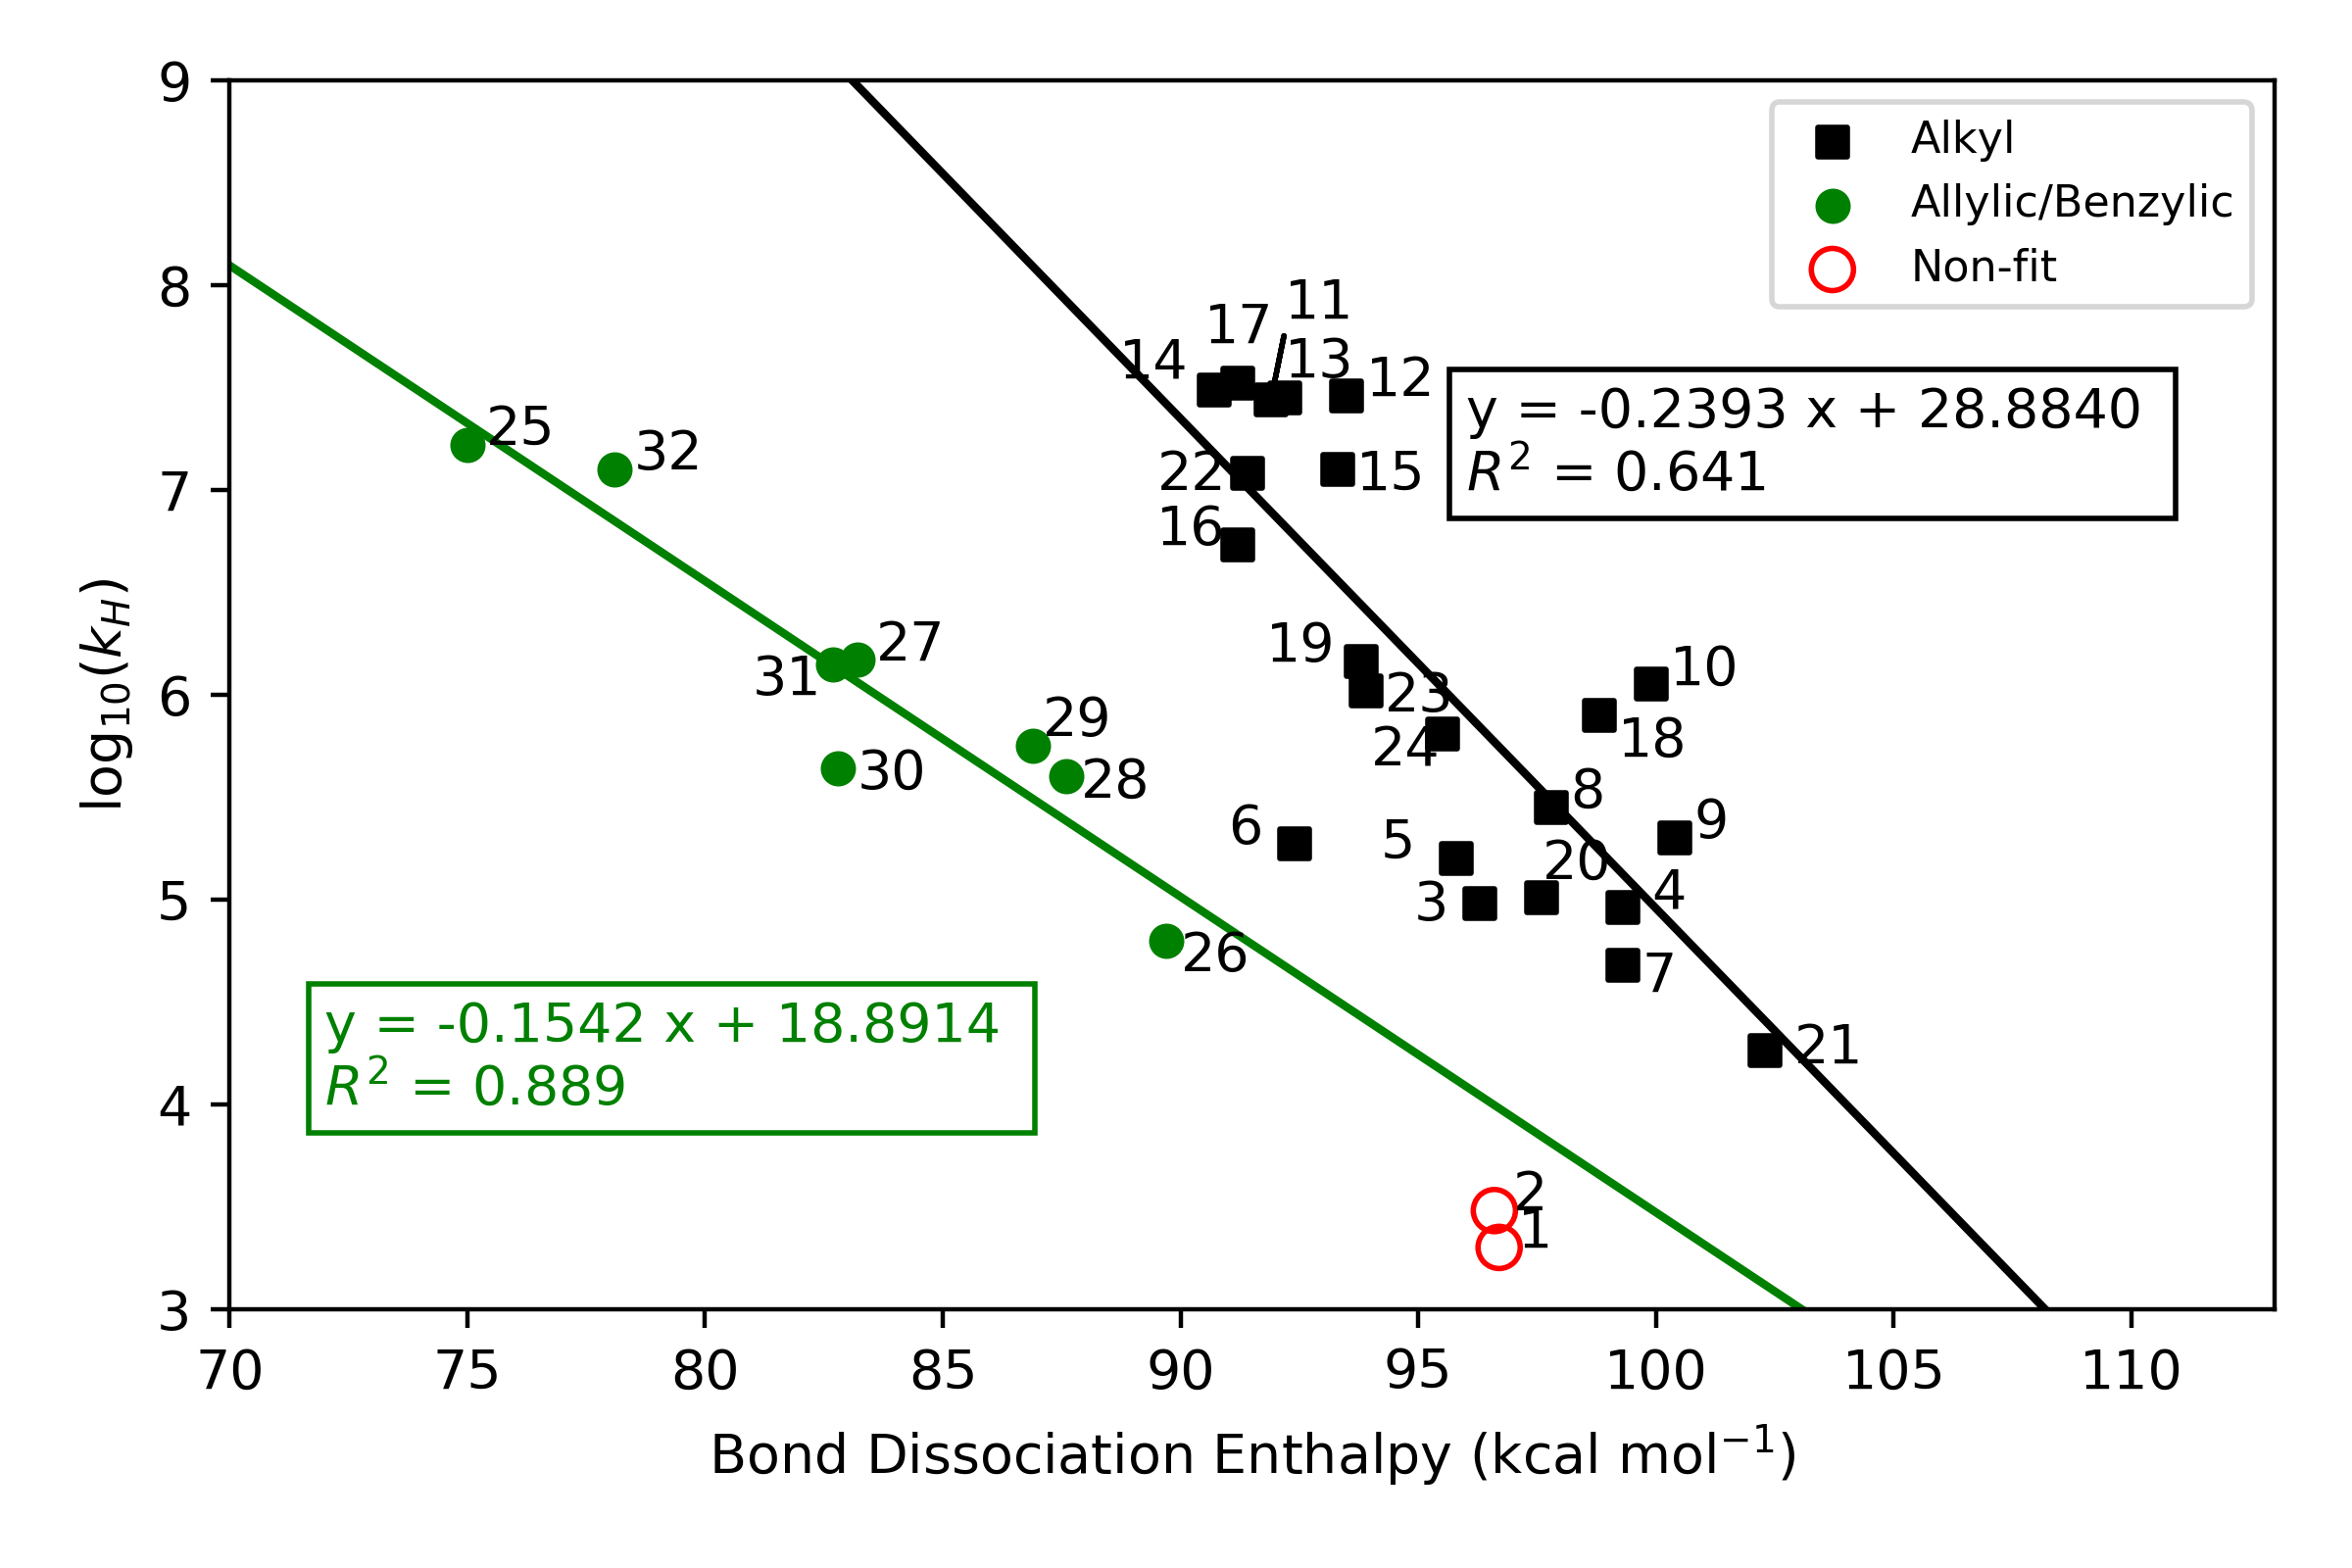
\includegraphics[width=\textwidth]{figures/bde-bep}
\begin{tabularx}{\textwidth}{| l X l X |}
  \hline
  1 & Acetone & 2 & Acetonitrile \\
  3 & Cyclopentane & 4 & Cyclohexane \\
  5 & Cycloheptane & 6 & Cyclooctane \\
  7 & 2,2-dimethylbutane & 8 & 2,3-dimethylbutane \\
  9 & Adamantane (2$^\circ$) & 10 & Adamantane (3$^\circ$) \\
  11 & Diethyl amine & 12 & Piperazine \\
  13 & Piperidine & 14 & Pyrrolidine \\
  15 & Morpholine & 16 & Propylamine \\
  17 & Triethylamine & 18 & 1,4-diazobicyclo[2.2.2]octane \\
  19 & Tetrahydrofuran & 20 & Dioxane \\
  21 & Dimethyl sulfoxide & 22 & Benzaldehyde \\
  23 & Hexamethylphosphoramide & 24 & Diethyl ether \\
  25 & 1,4-cyclohexadiene & 26 & Toluene \\
  27 & Benzyl alcohol & 28 & Ethylbenzene \\
  29 & Cumene & 30 & Diphenylmethane \\
  31 & Dibenzyl ether & 32 & 9,10-dihydroanthracene \\
  \hline
\end{tabularx}
  \caption[Bell-Evans-Polanyi plot of experimental rate constants (normalized
  for the number of equivalent hydrogen atoms) for HAT between \cumo\ and
  substrates against BDEs calculated using the ROCBS-QB3
  method.]{Bell-Evans-Polanyi plot of experimental rate constants (normalized
  for the number of equivalent hydrogen atoms) for HAT between \cumo\ and
  substrates against BDEs calculated using the ROCBS-QB3 method. Acetone and
  acetonitrile are note included in fitting as the experimental rate constants
  are approximate.} \label{fig:bde-bep}
\end{figure}

As with the experimental results in~\ref{fig:bep-expt}, there clearly exists
two distinct regions in~\ref{fig:bde-bep}. This is congruent with our initial
hypothesis that there should exist two linear relations: one for
allylic/benzylic C-H bonds, and another for alkyl C-H bonds. However, there
remains a considerable amount of scatter in the data, thus correlation of the
expected BEP relations is poor. For the allylic/benzylic series of C-H BDEs
which result in a radical which is delocalized, the coefficient of
determination is $R^2 = 0.89$. This result is consistent with work of Pratt et
al.\cite{Pratt2003}, which found a BEP plot $R^2 =0.82$ for the abstraction of
C-H bonds from models for unsaturated fatty acids. Most of the rate constants
used in the work of Pratt et al. are for the abstraction of \ch{C-H} by peroxyl
radicals, which were obtained through an experimental method that gives
estimated HAT rate constants with large associated errors. Thus, they suggested
that the degree of scatter is associated with experimental errors. The same
however cannot be said for the rate constants associated with this work.
Therefore, there may be additional physico-chemical factors at play.

The alkyl C-H BDEs show very weak correlation with \cumo\ HAT rate constants,
with an $R^2 =0.63$. One possibility is that applying the BEP principle to such
a large grouping of substrates is inappropriate. Thus, I have re-plotted this
data in~\ref{fig:bep-breakdown}, breaking the data into several smaller
chemical groupings: cyclic alkanes, other alkanes (branched and adamantane),
hydrogen bond donating (H-Bond Donors) species, and other \ch{C-H} bonds with
heteroatom neighbours (Het. Neighbours). Doing so appears to reveal one
reasonably well-correlated trend for \ch{C-H} bonds with heteroatom neighbours
($R^2 = 0.84$). There are two data points for the tertiary amines
(triethylamine and 1,4-diazobicyclo[2.2.2]octane\jnote{larger error in kH}),
which do not fit well with the expected trend, however it is unclear why they
do not fit into the other points in the heteroatomic neighbours trend.

Excluding points the tertiary amines results in an $R^2 = 0.92$.  The cyclic
alkanes are somewhat poorly correlated ($R^2 = 0.73$). Within the ``other
alkanes'' grouping consists of the two branched alkanes, 2,3-dimethylbutane and
2,2-dimethylbutane, as well as the secondary and tertiary \ch{C-H} positions of
adamantane. There may be a separate correlation for each of these, however
there are to few data points to explore this make this assertion. Extremely
poor correlation is observed for both the hydrogen bond donating species ($R^2
= 0.02$). This is likely due to the formation of a hydrogen bonded pre-reaction
complex that does not allow for HAT to occur without some subsequent
rearrangement. In general, there are no evident reasons on the basis of
group-additivity based arguments that explain the poor correlations observed.
Thus, the lack of simple relationships is perhaps evidence against the validity
of the BEP principle. However, before making any conclusions, we must consider
if there are any explanations that arise from examining the transition state
structures.

\begin{figure}[!htbp]
  \centering
  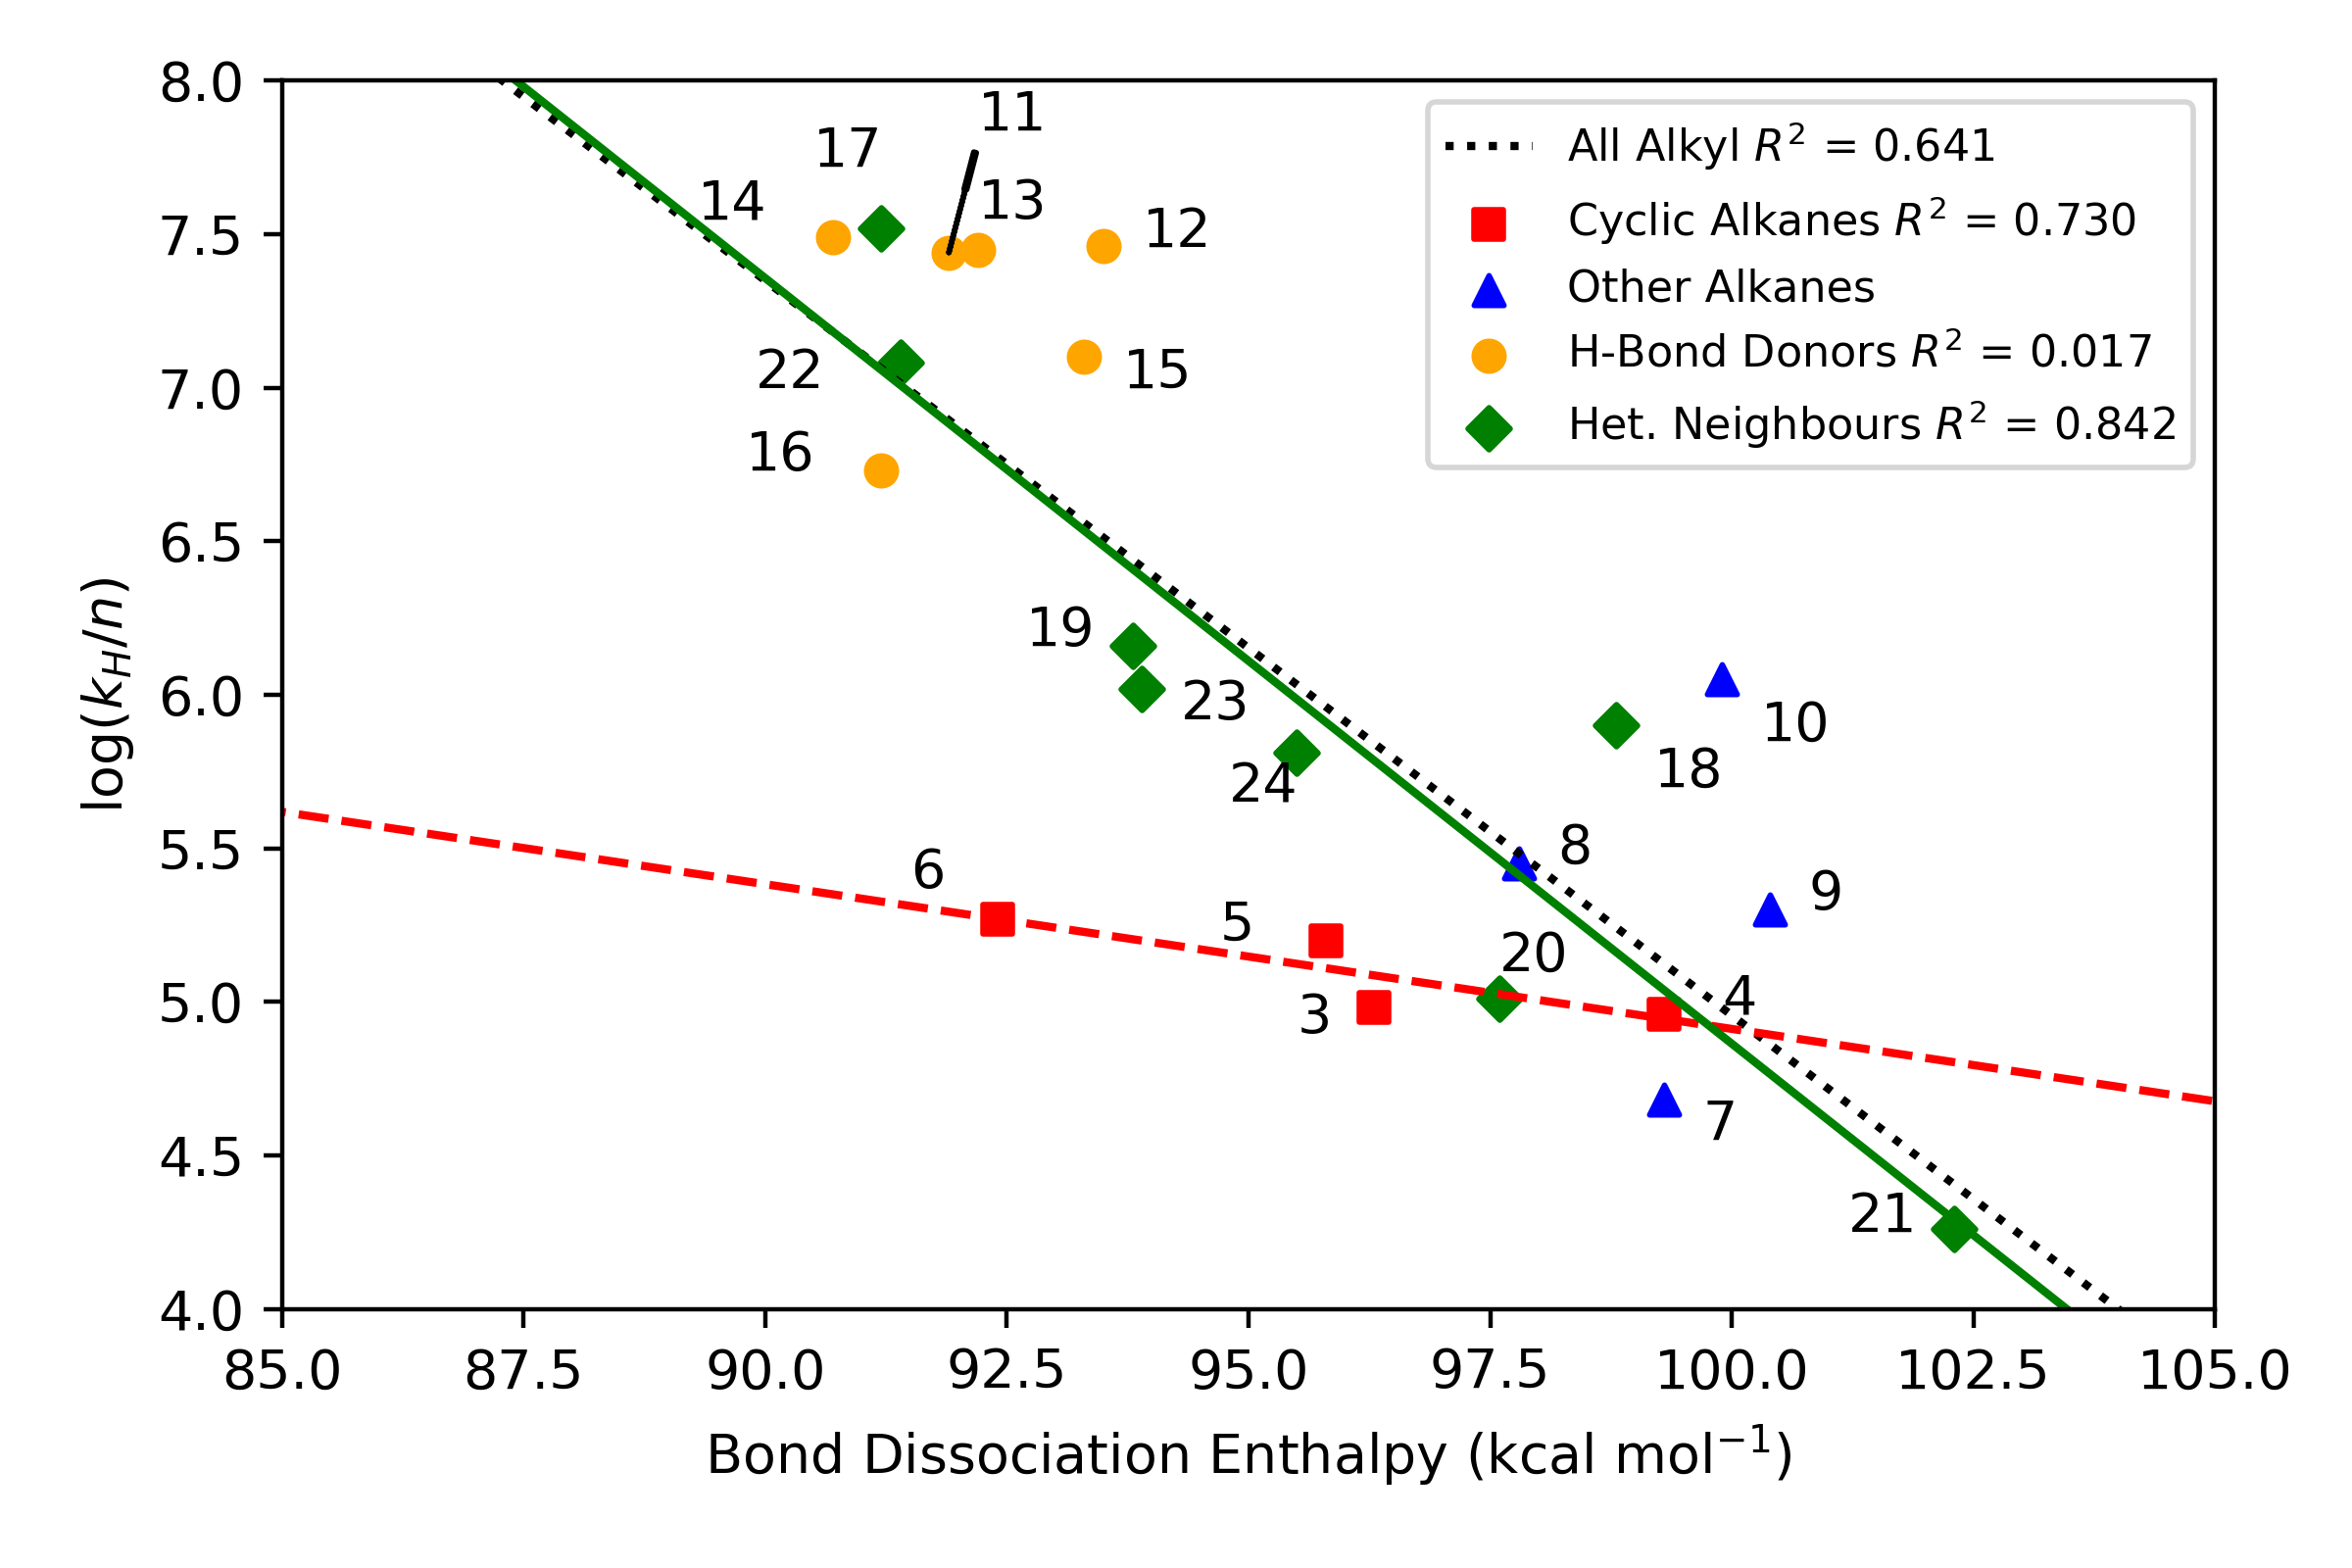
\includegraphics[width=\textwidth]{figures/bep-breakdown}
  \begin{tabularx}{\textwidth}{| l X l X |}
    \hline
    3 & Cyclopentane & 4 & Cyclohexane \\
    5 & Cycloheptane & 6 & Cyclooctane \\
    7 & 2,2-dimethylbutane & 8 & 2,3-dimethylbutane \\
    9 & Adamantane (2$^\circ$) & 10 & Adamantane (3$^\circ$) \\
    11 & Diethyl amine & 12 & Piperazine \\
    13 & Piperidine & 14 & Pyrrolidine \\
    15 & Morpholine & 16 & Propylamine \\
    17 & Triethylamine & 18 & 1,4-diazobicyclo[2.2.2]octane \\
    19 & Tetrahydrofuran & 20 & Dioxane \\
    21 & Dimethyl sulfoxide & 22 & Benzaldehyde \\
    23 & Hexamethylphosphoramide & 24 & Diethyl ether \\
    \hline
  \end{tabularx}
  \caption[Further breakdown of Bell-Evans-Polanyi plot of experimental rate
  constants (normalized for the number of equivalent hydrogen atoms) for HAT
  between \cumo\ and alkyl substrates against BDEs calculated using the
  ROCBS-QB3 method.]{Further breakdown of Bell-Evans-Polanyi plot of
  experimental rate constants (normalized for the number of equivalent hydrogen
  atoms) for HAT between \cumo\ and  substrates.} \label{fig:bep-breakdown}
\end{figure}

\newpage
\section{Transition state analysis}

In order to determine if there are any reasons for the breakdown of the BEP
principle, I have calculated TS structures for 20 of the reactions at the
B3LYP-D3(BJ)/6-311+G(2d,2p)//B3LYP-D3(BJ)/6-31+G$^*$ level of theory. Note that
the inclusion of the SMD continuum solvent model decreases the agreement in
calculated rate constant with experiment, and so gas-phase results are reported
herein (See Appendix~\ref{ap:bde},~\ref{fig:ap-kH-comp}). The experimental and
calculated HAT reaction rate constants ($k_H$) agree reasonably well (within 2
orders of magnitude) and are listed in~\ref{tab:ts-bep}, along with the
free-energy barrier heights ($\Delta G^\ddagger$) and the decomposition into
enthalpic and entropic terms: $\Delta G^\ddagger = \Delta H^\ddagger - T\Delta
S^\ddagger$.

\begin{table}[!htbp]
\caption[Reaction barrier heights for reactions of substrates with \cumo\
calculated in the gas phase at 298 K.]{Reaction barrier heights for reactions
of substrates with \cumo\ calculated in the gas phase at 298 K at the
B3LYP-D3(BJ)/6-311+G(2d,2p)//B3LYP-D3(BJ)/6-31+G$^*$ level of theory. Rate
constants are in units of \Ms, while all other values are in units of \kcalmol.
ID numbers match those in~\protect\ref{fig:bde-bep}. $^\dagger$TS structure
could not be fully optimized and contains a small additional imaginary
frequency.} \label{tab:ts-bep}
\hspace*{-1cm}
\begin{tabular}{l l c c c c c}
    ID & Substrate & $k_H (expt.) $ & $k_H (calc.)$ & $\Delta G^\ddagger$ & $\Delta H^\ddagger$ & $-T\Delta S^\ddagger$ \\
    \hline
    \multicolumn{7}{c}{\textbf{Excluded}}\\
    1 & Acetone      & $<$ 1\E{4} & 2.8\E{2} & 14.1 & 0.1 & 14.0 \\
    2 & Acetonitrile & $<$ 1\E{4} & 2.9\E{2} & 14.1 & 2.6 & 11.5 \\
    \hline
    \multicolumn{7}{c}{\textbf{Cyclic Alkanes}}\\
    3 & Cyclopentane$^\dagger$ & 9.5\E{5} & 5.5\E{4} & 11.0 & -2.0 & 13.0 \\
    4 & Cyclohexane            & 1.1\E{6} & 5.8\E{4} & 10.9 & -1.1 & 12.1 \\
    6 & Cyclooctane$^\dagger$  & 3.0\E{6} & 2.7\E{4} & 11.4 & -2.7 & 14.1 \\
    \hline
    \multicolumn{7}{c}{\textbf{Other Alkanes}}\\
    7 & 2,2-dimethylbutane      & 9.5\E{4} & 1.1\E{6} &  9.2 & -1.2 & 10.4 \\
    8 & 2,3-dimethylbutane      & 5.6\E{5} & 2.5\E{6} &  8.7 & -3.3 & 12.0 \\
    9 & Adamantane (2$^\circ$)  & 6.9\E{6} & 2.0\E{5} & 10.2 & -1.8 & 12.0 \\
    10 & Adamantane (3$^\circ$) & 6.9\E{6} & 1.1\E{7} &  7.9 & -3.9 & 11.8 \\
    \hline
    \multicolumn{7}{c}{\textbf{H-Bond Donor}} \\
    11 & Diethylamine                  & 1.1\E{8} & 8.2\E{9} & 3.9 & -9.1 & 13.0 \\
    \hline
    \multicolumn{7}{c}{\textbf{Heteroatom Neighbours}} \\
    18 & 1,4-diazobicyclo[2.2.2]octane & 9.6\E{6} & 5.1\E{7} & 6.9 & -5.3 & 12.3 \\
    20 & Dioxane                 & 8.2\E{5} & 1.2\E{7} &  7.8 & -4.0 & 11.8 \\
    21 & Dimethyl sulfoxide      & 1.8\E{4} & 2.7\E{4} & 11.4 & -0.5 & 11.9 \\
    22 & Benzaldehyde$^\dagger$  & 1.2\E{7} & 2.5\E{7} &  7.4 & -5.6 & 12.9 \\
    23 & Hexamethylphosphoramide & 1.9\E{7} & 3.9\E{7} &  7.1 & -7.3 & 14.4 \\
    24 & Diethyl ether           & 2.6\E{6} & 5.9\E{7} &  6.8 & -4.6 & 11.4 \\
    \hline
    \multicolumn{7}{c}{\textbf{Allylic/Benzylic}}\\
    25 & 1,4-cyclohexadiene               & 6.6\E{7} & 1.1\E{8} & 6.5 & -6.5 & 13.0 \\
    26 & Toluene                          & 1.8\E{5} & 2.0\E{5} & 10.2 & -3.5 & 13.7 \\
    29 & Cumene                           & 5.6\E{5} & 1.9\E{7} & 7.5 & -5.8 & 13.3 \\
    30 & Diphenylmethane$^\dagger$        & 8.7\E{5} & 1.8\E{6} & 8.9 & -5.6 & 14.5 \\
    32 & 9,10-dihydroanthracene$^\dagger$ & 5.0\E{7} & 2.2\E{8} & 6.1 & -8.5 & 14.6 \\
\end{tabular}
\end{table}

First, consider some general features associated with the TS complexes listed
in~\ref{tab:ts-bep}. One factor that may lead to deviations from the BEP
principle is the possibility for different HAT reaction mechanisms, i.e. direct
HAT or PCET. Consider first the reaction of toluene with \cumo. As this
reaction is similar to the self-exchange reaction of the benzyl-toluene couple
as described by DiLabio and Johnson,\cite{DiLabio2007} one might expect the
reaction to proceed via PCET. The lowest-energy TS complex has a partially
$\pi$-stacked conformation with the rings oriented approximately 40$^\circ$
relative to one another. Examination of the SOMO and HOMO reveals no
$\pi$-$\pi$ partial bonding interaction, as can be seen
in~\ref{fig:cumo-toluene}. The electron density of the SOMO is largely
localized on the toluene portion of the complex. This is likely due to the
additional non-conjugated carbon centre of \cumo, which prevents an additional
electron channel for PCET to occur. Therefore, this reaction takes place
through direct HAT, as has been previously described.\cite{Salamone2011} This
behaviour is specific to the \cumo\ radical, thus all the reactions likely also
take place through a direct HAT mechanism, and this should not factor into the
deviations in the observed BEP principle relationships.

\begin{figure}[!htbp]
\centering
\hspace*{-1.8cm}
\begin{minipage}{8cm}
  \centering
  \begin{overpic}[width=\textwidth]{figures/cumo-tol-somo}
  \put(5,100) {\large\textbf{A.}}
\end{overpic}
\end{minipage}%
\begin{minipage}{8cm}
  \centering
  \begin{overpic}[width=\textwidth]{figures/cumo-tol-homo}
  \put(5,100) {\large\textbf{B.}}
\end{overpic}
\end{minipage}
\caption[Structures of TS for HAT between \cumo\ and toluene with SOMO and
HOMO.]{Structures of TS for HAT between \cumo\ and toluene with \textbf{A.}
SOMO and \textbf{B.} HOMO. The elements are coloured as grey for carbon, white
for hydrogen, and red for oxygen. MOs are shown with an isovalue of 0.02
$e^-/$\AA.} \label{fig:cumo-toluene}
\end{figure}

For all of the TS structures of the reactions in~\ref{tab:ts-bep}, a
conformation that maximizes non-covalent interactions while minimizing steric
repulsion is adopted. In the cases of acetone, acetonitrile,
hexamethylphosphoramide (HMPA), and DMSO, a very weak hydrogen bonding
interaction is formed between the \ch{X=O} (or \ch{C+N} for acetonitrile)
moieties and the C-H of the methyl of \cumo. In all but two cases, this
involves a cisoid (partially-stacked) complex so that dispersion interactions
are maximized. The two outliers are benzaldehyde and cyclooctane. In order for
benzaldehyde to adopt a cisoid TS structure, there are two possibilities.
First, a T-shaped conformation could be adopted, rather than a slipped-parallel
$\pi$-stacked conformation. On the basis of the benzene-benzene non-covalently
bound dimer,\cite{Sinnokrot2002} this conformation is very slightly favourable
by circa 0.1 \kcalmol. However, this would require a rotation of nearly
90$^\circ$ of the \ch{C(CH3)2O^.} of \cumo, which has a predicted energetic
cost\footnotemark\ of 4.2 \kcalmol, and so this conformation is unlikely. On
the other hand, the \ch{C(CH3)2O^.} of \cumo\ could rotate to accommodate a
partially slipped-parallel $\pi$-stacking conformation in the TS complex. Note
that I was unable to obtain TS structures for either of the described possible
cisoid conformations for the benzaldehyde-\cumo\ TS complex, as geometry
optimization calculations did not converge. For cyclooctane, the difference in
free energy between the cisoid and transoid TS structures is 1.8 \kcalmol,
however both structures were unable to be fully optimized and contain a
secondary small imaginary frequency. The reason for the transoid TS structure
being more stable is somewhat unclear, but it is possible that the non-optimal
nature of the TS structures is the cause. Furthermore, it is possible that the
cyclooctane molecule undergoes a conformational change in forming the TS
complex which was not accounted for in these calculations. Cyclooctane has many
conformations that are close in relative energy.\cite{Dorofeeva1985}

\footnotetext{Calculated at the B3LYP-D3(BJ)/6-311+G(2d,2p) level of theory.}

TS complex structures and mechanism aside, there is one striking feature in the
reaction barriers calculated for HAT reactions involving \cumo: all the the
reactions studied are entropy-controlled at 298 K. This means that the
free-energy barrier, and thus rate constant, is controlled by the entropic
contributions, rather than the enthalpic contributions, i.e., $-T\Delta
S^\ddagger > \Delta H^\ddagger$. From the results in~\ref{tab:ts-bep}, it can
be said that $-T\Delta S^\ddagger >> \Delta H^\ddagger$ for hydrogen
abstraction by \cumo. One interpretation of these results is that \cumo\ is so
highly reactive that HAT is governed by trajectory, orientation, and degrees of
freedom, factors that are normally associated with the A-factor in Arrhenius
theory. In fact, in many cases, $\Delta H^\ddagger$ is calculated to be
negative with respect to the separated reactants. This implies that a
pre-reaction complex is formed, which, as was demonstrated in
Chapter~\ref{ch:arrhenius}, can have significance on HAT reactivity with
respect to the magnitude of the A-factor. Pre-reaction complex structures were
not calculated in this work, however, in some cases the systems have been
studied in combined experimental and theoretical work. Some examples of
previously calculated \cumo\ + substrate pre-reaction complex binding
enthalpies are: HMPA\footnotemark\ $\Delta H \approx$ -6 \kcalmol, DMSO $\Delta
H \approx$ -5 \kcalmol, and 1,4-diazobicyclo[2.2.2]octane
(DABCO)\cite{Salamone2011b} $\Delta H \approx$ -0.1 \kcalmol. Note that the
calculated enthalpic barrier herein is -5.3 \kcalmol\ for DABCO, a result that
can be ascribed to differences in computational methods. In
Ref.~\citenum{Salamone2011b}, no dispersion correction was used, thus
accounting for a less stable TS complex and pre-reaction complex. The
calculated difference in enthalpy from pre-reaction complex to TS complex for
DABCO was found to be only 1.0 \kcalmol.

\footnotetext{DMSO and HMPA were studied in Ref. \citenum{Salamone2012} at the
B3LYP-DCP\cite{Torres2012}/6-31+G(2d,2p) level of theory}

The fact that hydrogen abstraction by \cumo\ is entropy-controlled is perhaps
unsurprising, given the work of \citet{Finn2004}, which demonstrated that HAT
reactions involving various organic substrates and the closely related radical
\ch{$t$-BuO^.} are also entropy-controlled at room temperature. Furthermore, it
has been shown that \cumo\ and \ch{$t$-BuO^.} display very similar hydrogen
atom abstraction reactivities.\cite{Salamone2011, Valgimigli1995, Sheeller2001,
Baignee1983} It is surprising then that these radicals remain so often applied
as proxies for reactive oxygen species in kinetic studies. Future work should
use extreme caution in applying \cumo\ and \ch{$t$-BuO^.} as chemical probes,
as been noted in the past.\cite{Finn2004, Salamone2011b, Salamone2011} Note
also that it is uncommon to encounter entropy-controlled reactions in organic
chemistry, and they are often associated with non-Arrhenius behaviour. Other
examples of reported entropy-controlled reactions include the addition of a
carbene across a multiple bond,\cite{Houk1984, Moss2017} and radical-radical
recombination reactions.\cite{Sobek2001}

Classical physical organic chemical literature can explain why the reactions
which are entropy-controlled do not follow ``normal'' LFERs.\cite{Exner1973}
\citet{Blackadder1958} defined three classifications for different types of
LFERs, the first of which applies to the BEP principle: A series of reactions
with constant entropy are controlled by enthalpy changes that are based on
electronic effects that do not affect the form of the TS. Therefore, reaction
rates that involve non-isoentropic TS complex formation will not correlate with
bond strengths, as is observed herein. It seems prudent at this point to
suggest that expecting reactions to be isoentropic with respect to transition
state formation is an over-simplification, especially given the number of
factors that contribute to entropy in solvent phase chemistry.

\section{Is the Bell-Evans-Polanyi principle valid?}

The question still remains whether the BEP principle is valid or not. Recall
from Equation~\ref{eq:Ea-vs-dH} that $E_a$ is related directly to $\Delta
H^\ddagger$. Thus, if the BEP principle still holds for HAT reactions between
\cumo\ and organic substrates, then the calculated values of $\Delta
H^\ddagger$ should be a function of \ch{C-H} BDE. These data are plotted
in~\ref{fig:bep-dG}.

\begin{figure}[!htbp]
  \centering
  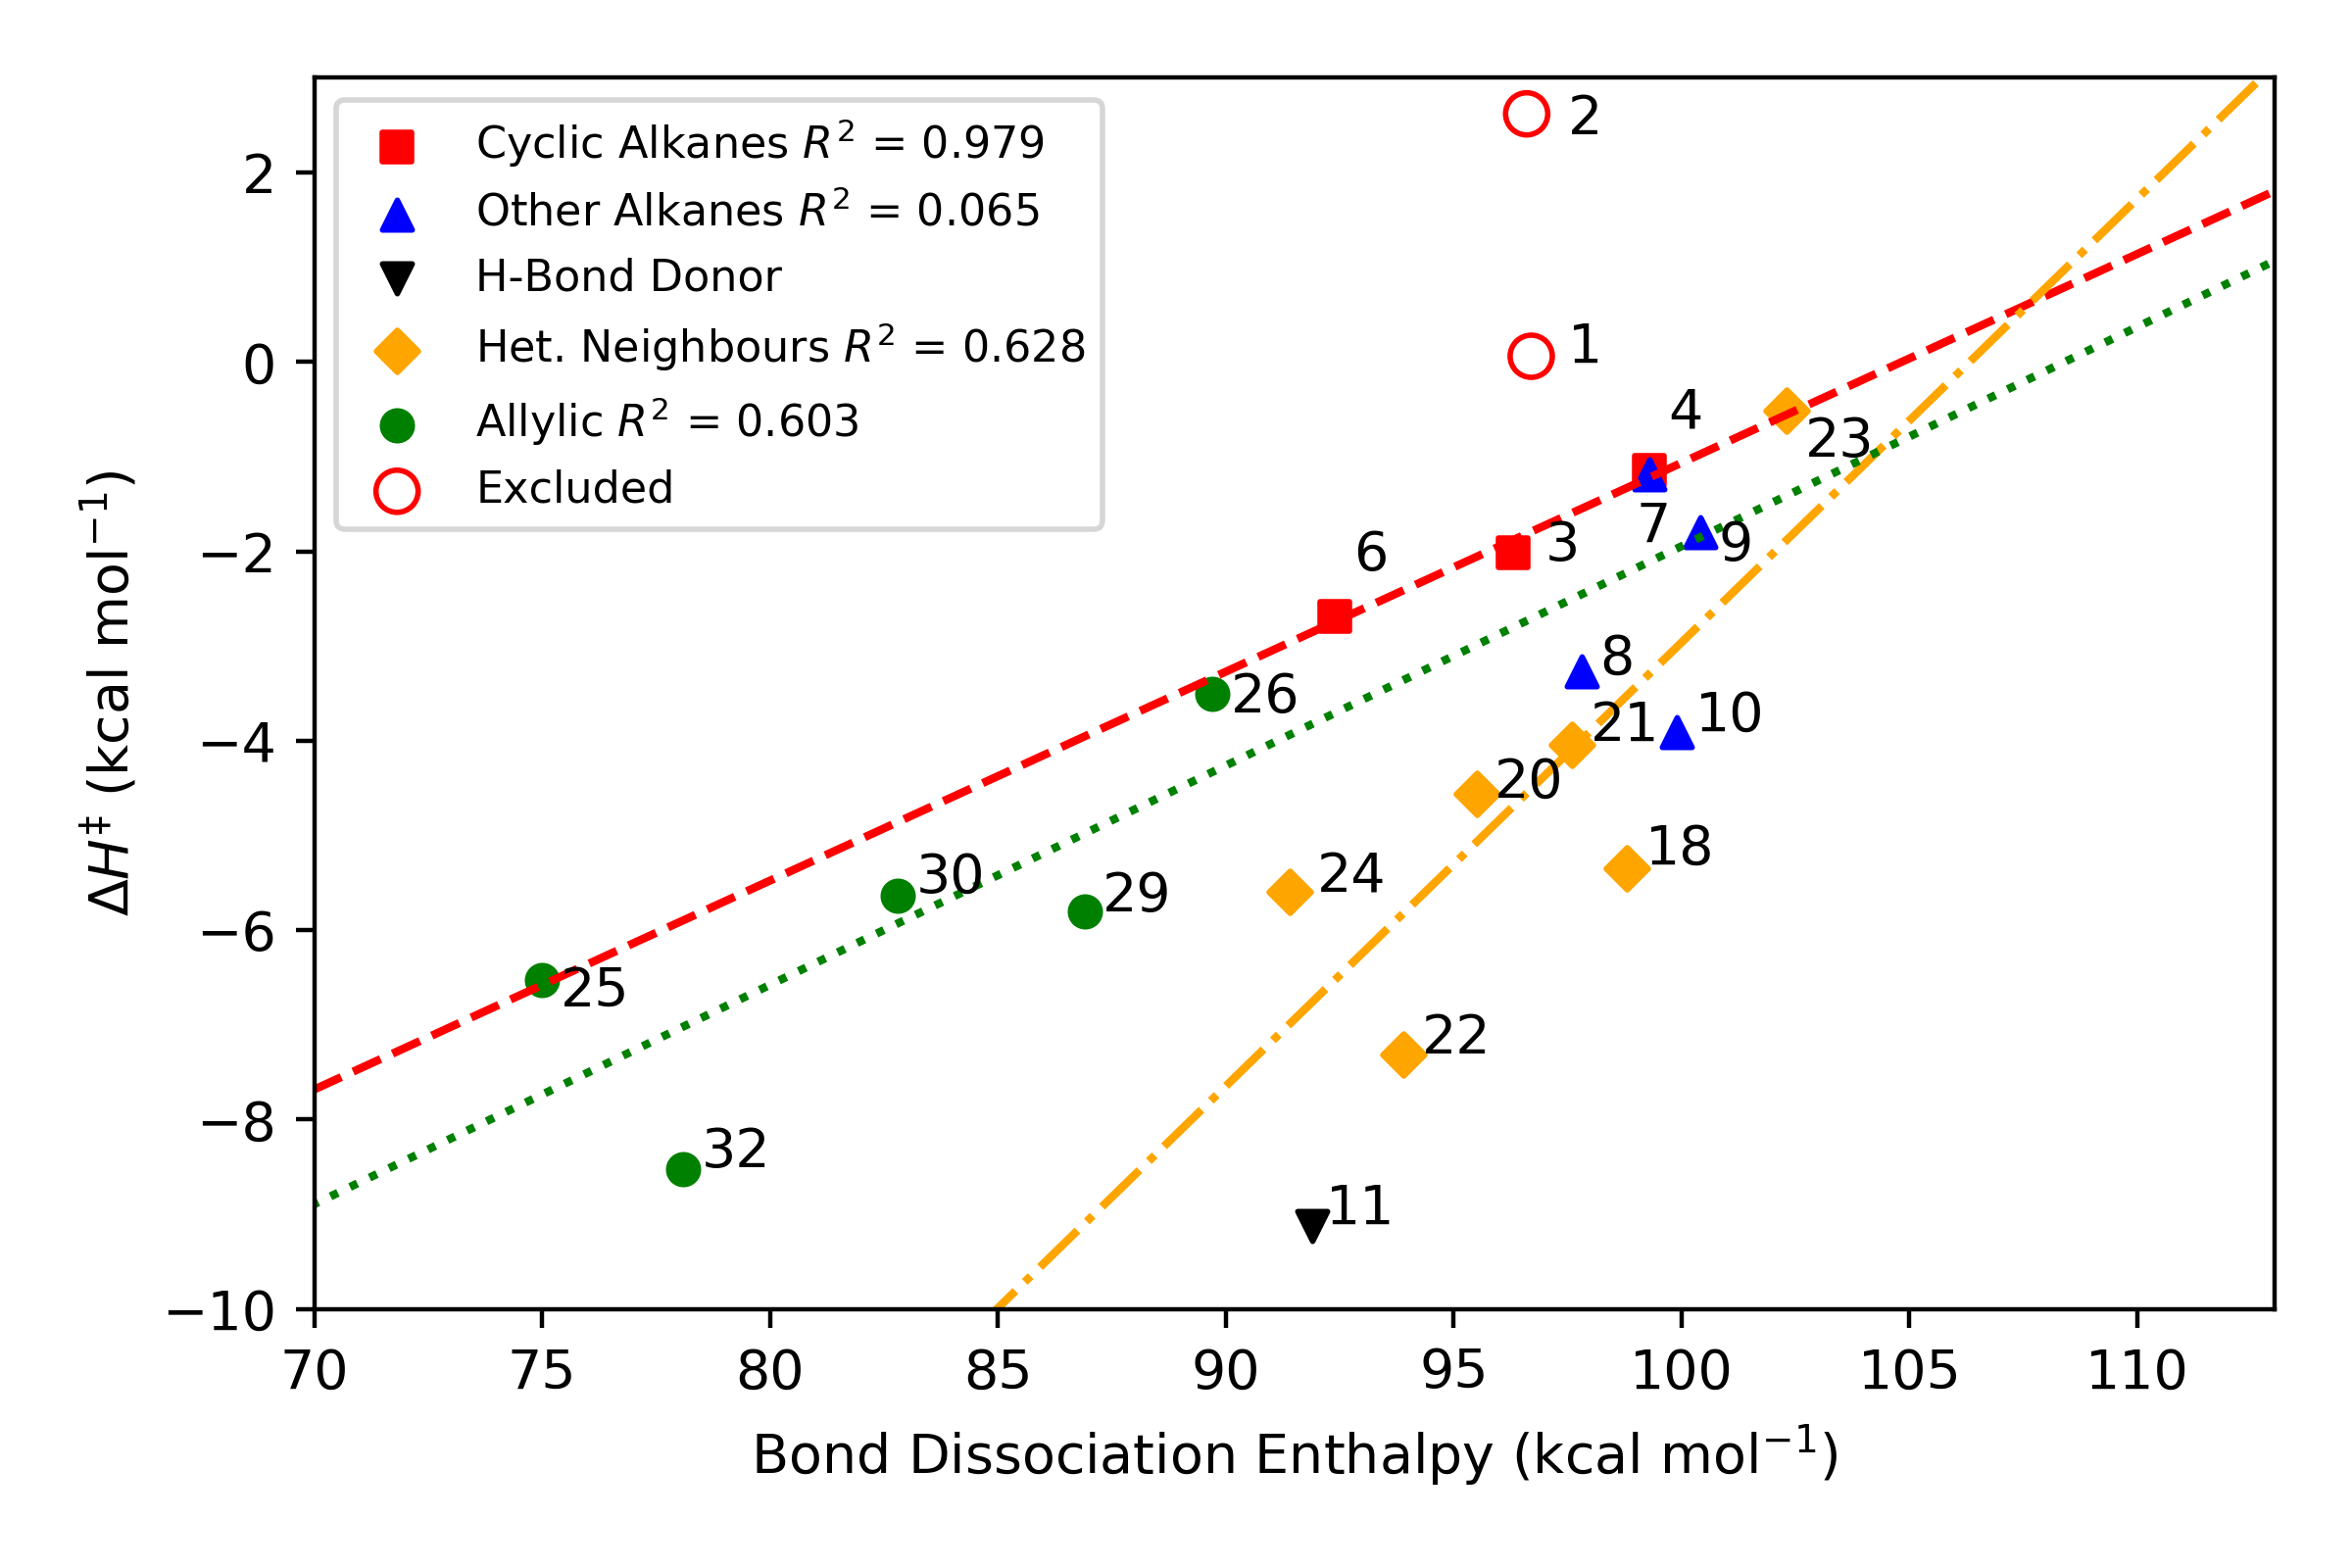
\includegraphics[width=\textwidth]{figures/bep-dG}
\begin{tabularx}{\textwidth}{| l X l X |}
  \hline
  1 & Acetone & 2 & Acetonitrile \\
  3 & Cyclopentane & 4 & Cyclohexane \\
  6 & Cyclooctane & 7 & 2,2-dimethylbutane \\
  8 & 2,3-dimethylbutane & 9 & Adamantane (2$^\circ$) \\
  10 & Adamantane (3$^\circ$) & 11 & Diethyl amine \\
  18 & 1,4-diazobicyclo[2.2.2]octane & 20 & Dioxane \\
  21 & Dimethyl sulfoxide & 22 & Benzaldehyde \\
  23 & Hexamethylphosphoramide & 24 & Diethyl ether \\
  25 & 1,4-cyclohexadiene & 26 & Toluene \\
  29 & Cumene & 30 & Diphenylmethane \\
  32 & 9,10-dihydroanthracene & & \\
  \hline
\end{tabularx}
\caption{Bell-Evans-Polanyi plot of calculated enthalpic barriers for HAT
between \cumo\ and substrates against BDEs calculated using the ROCBS-QB3
method.} \label{fig:bep-dG}
\end{figure}

Perhaps unsurprisingly at this point, there is once again a great deal of
scatter in the data. The cyclic alkanes fit into a linear relationship that is
very well correlated ($R^2$ = 0.98). However, all other chemical groupings show
very poor correlation. Therefore, the correlation seen for the cycloalkanes is
an adventitious example of the BEP principle showing a linear relation between
$\Delta H^\ddagger$ and BDE. Even the substrates with allylic/benzylic \ch{C-H}
bonds show only weak correlation in a BEP relation ($R^2 = 0.63$), although the
experimental results show a reasonable correlation between $\log(k_H/n)$ and
calculated BDEs. Therefore, the experimental results are likely serendipitous,
especially considering the reactions are entropy-controlled and
non-isoentropic.

Further analysis of the allylic/benzylic relation demonstrates a clear
breakdown in the BEP principle. If one begins with toluene with a BDE of 89.7
\kcalmol\ and $\Delta H^\ddagger$ of -3.5 \kcalmol, then the addition of two
methyl substituents forms cumene, with a BDE of 86.9 \kcalmol\ and $\Delta
H^\ddagger$ of -5.8 \kcalmol, indicating the stabilization of the TS by
substituents. However, if one adds another phenyl group instead of two methyl
groups, diphenylmethane is obtained, which has a BDE of 82.8 \kcalmol. This
indicates that phenyl is a better radical stabilizing group, however $\Delta
H^\ddagger$ is -5.6 \kcalmol, which is slightly higher than that of cumene. The
difference can be partially attributed then to differences in progress along
the reaction coordinate. Evidence of this difference is the spin density
localized on the O-centre of \cumo\ in the TS complex, which should go to zero
as the reactants move to products. The \ch{O^.} spin densities are 0.477 $e^-$,
0.528 $e^-$, and 0.518 $e^-$ for toluene, cumene, and diphenylmethane,
respectively. Therefore, the progress along the reaction coordinate is furthest
for toluene, and progressively less far for diphenylmethane and cumene. Note,
that the \ch{O^.} spin densities for cyclopentane, cyclohexane, and cyclooctane
are 0.455 $e^-$, 0.452 $e^-$, and 0.458 $e^-$, respectively. Therefore the
progress along the reaction coordinate for the cycloalkanes is roughly the
same.

Such contradictory data makes it very difficult to draw any conclusions.
Instead, I shall make some suggestions as to why the BEP principle is an
incomplete theoretical construct for describing the HAT reaction of \cumo\ with
organic substrates:

\begin{enumerate}
  \item HAT reactions between \cumo\ and these organic substrates may be
	  decidedly exothermic, resulting in reactions with no enthalpic
	  barrier associated with the breaking of a \ch{C-H} bonds and the
	  formation of an \ch{O-H} bond. This is supported by the fact that the
	  calculated enthalpic barriers are all very low or even negative.
	  Therefore, any remaining nominal activation energy is a result of
	  stereo-electronic interactions between \cumo\ and the substrate.
	  Also, the high reactivity of \cumo\ also suggests that abstraction
	  from the weakest bond in a substrate will not always occur.  The site
	  of abstraction will most likely be determined by the orientation of
	  the substrate upon collision. This is likely an additional reason why
	  $\log{k_H/n}$ does not correlate with the calculated \ch{C-H} BDEs.

  \item Polar effects have been shown to be extremely important in the
	  stability of the TS complex.\cite{Roberts1999} The species involved
	  in HAT reactions are often neutral radicals, thus the influence of
	  charge transfer in the TS complex can have important implications.
	  Consider the TS of a generic HAT reaction in~\ref{fig:hatts}, there
	  are four obvious resonance forms. Oxygen-centred radicals are
	  electrophilic in nature, thus the importance of the third resonance
	  structure increases. The BEP principle does not account for polarity
	  in the TS complex, as these effects are not captured by the BDE of
	  the substrate, thus $\Delta H^\ddagger$ does not correlate well with
	  BDE. This issue was addressed by \citet{Roberts1994}, who suggested
	  an extension of the BEP principle to include simple empirical
	  parameters that capture the polar effects in the transition state.

  \begin{scheme}[!htbp]
    {\huge\ch{[X-H-Y]}$^\ddagger$} \\
    \vspace{0.5cm}
    {\large
    \ch{[X^.H-Y]}$^\ddagger$ \ch{<-> [X-H Y^.]}$^\ddagger$ \ch{<->
      [X:^-H^.Y^+]}$^\ddagger$ \ch{<-> [X^+H^.Y:^-]}$^\ddagger$}
    \caption{A generic HAT transition state structures and possible resonance forms.}
  \label{fig:hatts}
  \end{scheme}

\item The BEP principle is an over-simplification that does not capture nearly
enough of the physics associated with the deceptively complex hydrogen
abstraction reactivity of \cumo\ (or \ch{$t$-BuO^.}). Therefore, I suggest that
the BEP principle should not be used as a tool for predicting activation
energies or rate constants. One method that has been popularized by Mayer is
the use of Marcus cross-relations.\cite{Mayer2010} This predictive method has
also been used to explain reactions that have negative enthalpic
barriers.\cite{Mader2004} An alternative approach is that of Zavitsas, that
predicts activation energies based on so-called ``triplet
repulsion''\footnotemark\ and radical delocalization.\cite{Zavitsas1995,
Zavitsas2012} It is clear from the analysis herein that the BEP principle is
valid only as a conceptual framework, rather than a true linear relationship.
\end{enumerate}

\footnotetext{Zavitsas uses the term ``triplet repulsion'' to  describe
repulsion between the parallel spins of the hydrogen atom acceptor and donor
atoms ($\uparrow\downarrow\uparrow$ or $\downarrow\uparrow\downarrow$) in the
TS complex.}
